% ------------------------------------------------------------------------
% Ph.D. Thesis Defended on
% ------------------------------------------------------------------------

%--------------------------------------------------------------------------
%%From: Jose Angel Castellanos <joseac@robot3.cps.unizar.es>

%%Modificado por: José Merseguer y posteriormente por Jorge Júlvez

\documentclass[twoside,a4]{book}
%\usepackage{psfig}
%\usepackage{latexsym}
%\usepackage[english]{babel}
%\usepackage{ifthen}
\usepackage{graphicx}
%\usepackage[centertags]{amsmath}
\usepackage{amsmath}
\usepackage{amsfonts}
%\usepackage{amssymb}
\usepackage{amsthm}
%\usepackage{newlfont}
%\usepackage{sty/PNotation}
\usepackage{psfrag}%para reemplazar textos en una figura por formulas
\usepackage[ps2pdf]{hyperref}
\usepackage{subfigure}
%\usepackage{tabularx}
%\usepackage{makeidx}
\sloppy % para que nunca se pase de la raya (al final de cada lnea)

\renewcommand{\topfraction}{10.0}
\setcounter{topnumber}{1}
\renewcommand{\bottomfraction}{0.0}
\setcounter{totalnumber}{1}
\renewcommand{\arraystretch}{1.25}
%\renewcommand{\baselinestretch}{1.21}
\renewcommand{\baselinestretch}{1.11}

%\renewcommand{\textfraction}{0.25}
%\renewcommand{\floatpagefraction}{0.75}
%\setlength{\textheight}{18.8cm} \setlength{\textwidth}{13cm}
%\setlength{\topmargin}{3cm} \setlength{\oddsidemargin}{0.5cm}
%\setlength{\evensidemargin}{2.3cm}

\makeatletter
  \long\def\@makecaption#1#2{
  \vskip 10pt
  \setbox\@tempboxa\hbox{\small{\bf #1}: #2}
  \ifdim \wd\@tempboxa >\hsize {\small{\bf #1}: #2}\par \else \hbox
  to\hsize{\hfil\box\@tempboxa\hfil}
  \fi}
\makeatother

\makeatletter \if@twoside
  \def\ps@headings{%
      \let\@oddfoot\@empty\let\@evenfoot\@empty
      \def\@evenhead{\thepage\hfil\slshape\leftmark}%
      \def\@oddhead{{\slshape\rightmark}\hfil\thepage}%
      \let\@mkboth\markboth
    \def\chaptermark##1{%
      \markboth {{%
        \ifnum \c@secnumdepth >\m@ne
          \if@mainmatter
            \@chapapp\ \thechapter. \ %
          \fi
        \fi
        ##1}}{}}%
    \def\sectionmark##1{%
      \markright {{%
        \ifnum \c@secnumdepth >\z@
          \thesection. \ %
        \fi
        ##1}}}}
\else
  \def\ps@headings{%
    \let\@oddfoot\@empty
    \def\@oddhead{{\slshape\rightmark}\hfil\thepage}%
    \let\@mkboth\markboth
    \def\chaptermark##1{%
      \markright {{%
        \ifnum \c@secnumdepth >\m@ne
          \if@mainmatter
            \@chapapp\ \thechapter. \ %
          \fi
        \fi
        ##1}}}}
\fi
\def\ps@myheadings{%
    \let\@oddfoot\@empty\let\@evenfoot\@empty
    \def\@evenhead{\thepage\hfil\slshape\leftmark}%
    \def\@oddhead{{\slshape\rightmark}\hfil\thepage}%
    \let\@mkboth\@gobbletwo
    \let\chaptermark\@gobble
    \let\sectionmark\@gobble
    }
\makeatother \pagestyle{headings}

% Redefinicion de los encabezamientos (estilo Laura)

\RequirePackage{fancyhdr}

\renewcommand{\headrulewidth}{0.5pt}
\renewcommand{\chaptermark}[1]{\markboth{\thechapter. #1}{}}
\renewcommand{\sectionmark}[1]{\markright{\thesection. #1}}
%\fancyhead[RE]{\slshape \nouppercase\leftmark}
%\fancyhead[LO]{\slshape \nouppercase\rightmark}
%\fancyhead[LE,RO]{\thepage}
%\cfoot{\fancyplain{\textrm{\thepage}}{}}
 % estilo Merse

% Math commands


\theoremstyle{definition}
\newtheorem{thm}{Theorem}[chapter]
\newtheorem{cor}[thm]{Corollary}
\newtheorem{lem}[thm]{Lemma}
\newtheorem{prop}[thm]{Proposition}
\newtheorem{pro}[thm]{Property}
\newtheorem{defn}[thm]{Definition}
\newtheorem{algo}[thm]{Algorithm}

% Net commands
% Math commands

\def\b#1{\mathchoice{\hbox{\boldmath $\displaystyle #1$}}
        {\hbox{\boldmath $\textstyle #1$}}
        {\hbox{\boldmath $\scriptstyle #1$}}
        {\hbox{\boldmath $\scriptscriptstyle #1$}}}

\newcommand{\preset}[1]{\ensuremath{\,\!^\bullet{#1}}}
\newcommand{\postset}[1]{\ensuremath{{#1}^\bullet}}
\newcommand{\vect}[1]{{\ensuremath{\mathbf{#1}}}}
\newcommand{\acr}[1]{{\ensuremath{\mathrm{#1}}}}             % acronyms and log-like functions
\newcommand{\oddvect}[1]{\ensuremath{\boldsymbol{#1}}}     % odd vectors (e.g. greek letter)
\newcommand{\enab}{\acr{enab}}
\newcommand{\la}{\ensuremath{\b{\lambda}}}  % lambda
\newcommand{\Pre}{\b{Pre}}                  % the preincidence matrix
\newcommand{\Post}{\b{Post}}                % the postincidence matrix
\newcommand{\C}{\b{C}}                      % the incidence matrix
\newcommand{\m}{\b{m}}                      % a marking
\newcommand{\mk}{\b{m}}                      % a marking
\newcommand{\vf}{\b{f}}                     % continuous flow
\newcommand{\vy}{\b{y}}                     % a P-semiflow
\newcommand{\vv}{\b{v}}                     % vector of visit ratios
\newcommand{\si}{\ensuremath{\sigma}}          % a firing sequence
\newcommand{\vsi}{\oddvect{\si}}               % its firing count vector
\newcommand{\spbar}{\mbox{$\: \mid \;$}} % a spaced bar, for set definitions, etc.
\newcommand{\zeros}{\b{0}}                              % vector 0
\newcommand{\mo}{\b{m}_0}                   % the initial marking
\newcommand{\nat}{\mathbb{N}}
\newcommand{\inte}{\mathbb{Z}}
\newcommand{\raz}{\mathbb{Q}}
\newcommand{\rea}{\mathbb{R}}
\newcommand{\comp}{\mathbb{C}}
\newcommand{\imm}{\mathbb{I}}
\newcommand{\myquote}[1]{\textquotedblleft{#1}\textquotedblright}   % quotation
\newcommand{\N}{{\ensuremath{\mathcal{N}}}}    % a net
\newcommand{\sys}{\ensuremath{\langle\N ,\b{m_0}\rangle}} % system (N,mo)
\newcommand{\tN}{\ensuremath{\langle\N ,\b{\lambda} \rangle}} % timed-net (N,Lambda)
\newcommand{\tsys}{\ensuremath{\langle\N ,\b{\lambda}, \b{m_0}\rangle}} % timed-system (N,Lambda,mo)
\newcommand{\support}[1]{\ensuremath{\|{#1}\|}}            % support of an array

%-------------------------------------------------------------------------
\def\chaptername{Section}
\usepackage{color,verbatim}
%\nofiles %no genera el fichero toc, asi utilizo uno donde la num de la Bibliografia este correcta
%\makeindex
\usepackage{amsmath}
\begin{document}

% ------PRELIMINARES ---------------------------------------------------------

\pagestyle{empty}


\noindent

\vfill

\includegraphics[scale=2]{figs/uz-w.eps} \hspace{5cm}  
\includegraphics[scale=1.8]{figs/diis-c.eps}
\begin{center}
    \Large

\end{center}

\vfill
\begin{center}
    \Large

\end{center}

\vfill
\begin{center}
    \Huge
    SimHPN: A MATLAB Toolbox for Hybrid Petri Nets\\
\end{center}

\begin{center}
\Large
    - USER MANUAL v. 1.0-\\
\end{center}


\vfill
\begin{center}
    \Large

\end{center}
\begin{center}
   \Large
   Jorge J\'ulvez and Cristian Mahulea
\end{center}


\vfill
\begin{center}
    \Large

\end{center}




\begin{center}
\Large
    Dept. of Computer Science and Systems Engineering\\
    University of Zaragoza\\
\end{center}


\vfill
\begin{center}
\Large

\end{center}



\begin{center}
\Large
    January 2012
\end{center}




\cleardoublepage

\frontmatter  % pone numeros romanos, etc.



\pagestyle{fancy}

\tableofcontents

\cleardoublepage
%---CAPITULOS ----------------------------------------------------------------

\mainmatter  %pone numeros arabigos, etc.

\def\chaptermark#1{\markboth{\thechapter.\ #1}{}}
\def\sectionmark#1{\markright{\thesection.\ #1}}

\graphicspath{{figs/}}

% RESUMEN

\chapter{Overview}
%\addcontentsline{toc}{chapter}{Overview}
%\markboth{Overview}{Overview}


Petri nets (PNs)\cite{ARMura89,BODHPSV93} is a mathematical formalism for the description of discrete-event systems, that has been successfully used for modeling, analysis and synthesis purposes of such systems. A key feature of a
PN is that its structure can capture graphically fundamental primitives in concurrency theory such as parallelism,
synchronization, mutual exclusion, etc. The state of a PN system is given by a vector of non-negative
integers representing the marking of its places.

As any other formalism for discrete event systems, PNs suffer from the \emph{state explosion problem} which produces an exponential growth of the size of the state space with respect to the initial marking. One way to avoid the state explosion is to relax the integrality constraint in the firing of transitions and deal with transitions that are fired in real amounts. A transition whose firing amount is allowed to be any real number between zero and its enabling degree is said to be a \emph{continuous transitions}. The firing of a continuous transition can produce a real, not integer, number of tokens in its input and output places. If all transitions of a net are continuous, then the net is said to be continuous. If a non-empty proper subset of transitions is continuous, then the net is said to be hybrid \cite{BODavid10}.

Different time interpretations can be considered for the firing of continuous transitions. The most popular ones are infinite and finite server semantics which represent a first order approximation of the firing frequency of discrete transitions. For a broad class of Petri nets, infinite server semantics offers a better approximation of the steady-state throughput  than finite server semantics \cite{ARMARESI09}. Moreover, finite server semantics can be exactly mimicked by infinite server semantics in discrete transitions simply by adding a self-loop place. A third firing semantics, called product semantics, is also frequently used when dealing with biochemical and population dynamics systems.

$SimHPN$ is a MATLAB embedded software that provides support for infinite server and product semantics in both, discrete and continuous, types of transition. A description of a preliminary version of this software can be found in~\cite{JuMa10,JuMaVa11,simhpn2012806}. This is the first MATLAB package that enables the analysis and simulation of hybrid nets with these two firing semantics. There already exists a toolbox dealing with discrete Petri nets~\cite{IPMaMaPa03c}, and one for the so-called first order hybrid Petri nets~\cite{ICSeGiSe08} which provides support for continuous transitions under finite server semantics. The main features of the $SimHPN$ toolbox are: 
\begin{enumerate}
\item simulation of hybrid Petri nets under different server semantics; 
\item computation of steady state throughput bounds; 
\item computation of minimal P-T \emph{semiflows}; 
\item optimal sensor placement;
\item  optimal control algorithm; 
\item import models from different graphical Petri net editors.
\end{enumerate}

Figure \ref{f-main} shows the Graphical user Interface of SimHPN automatically opened in MATLAB once 

\texttt{>> SimHPN} 

command is executed at the command prompt. 

\begin{figure}
   \centering{
   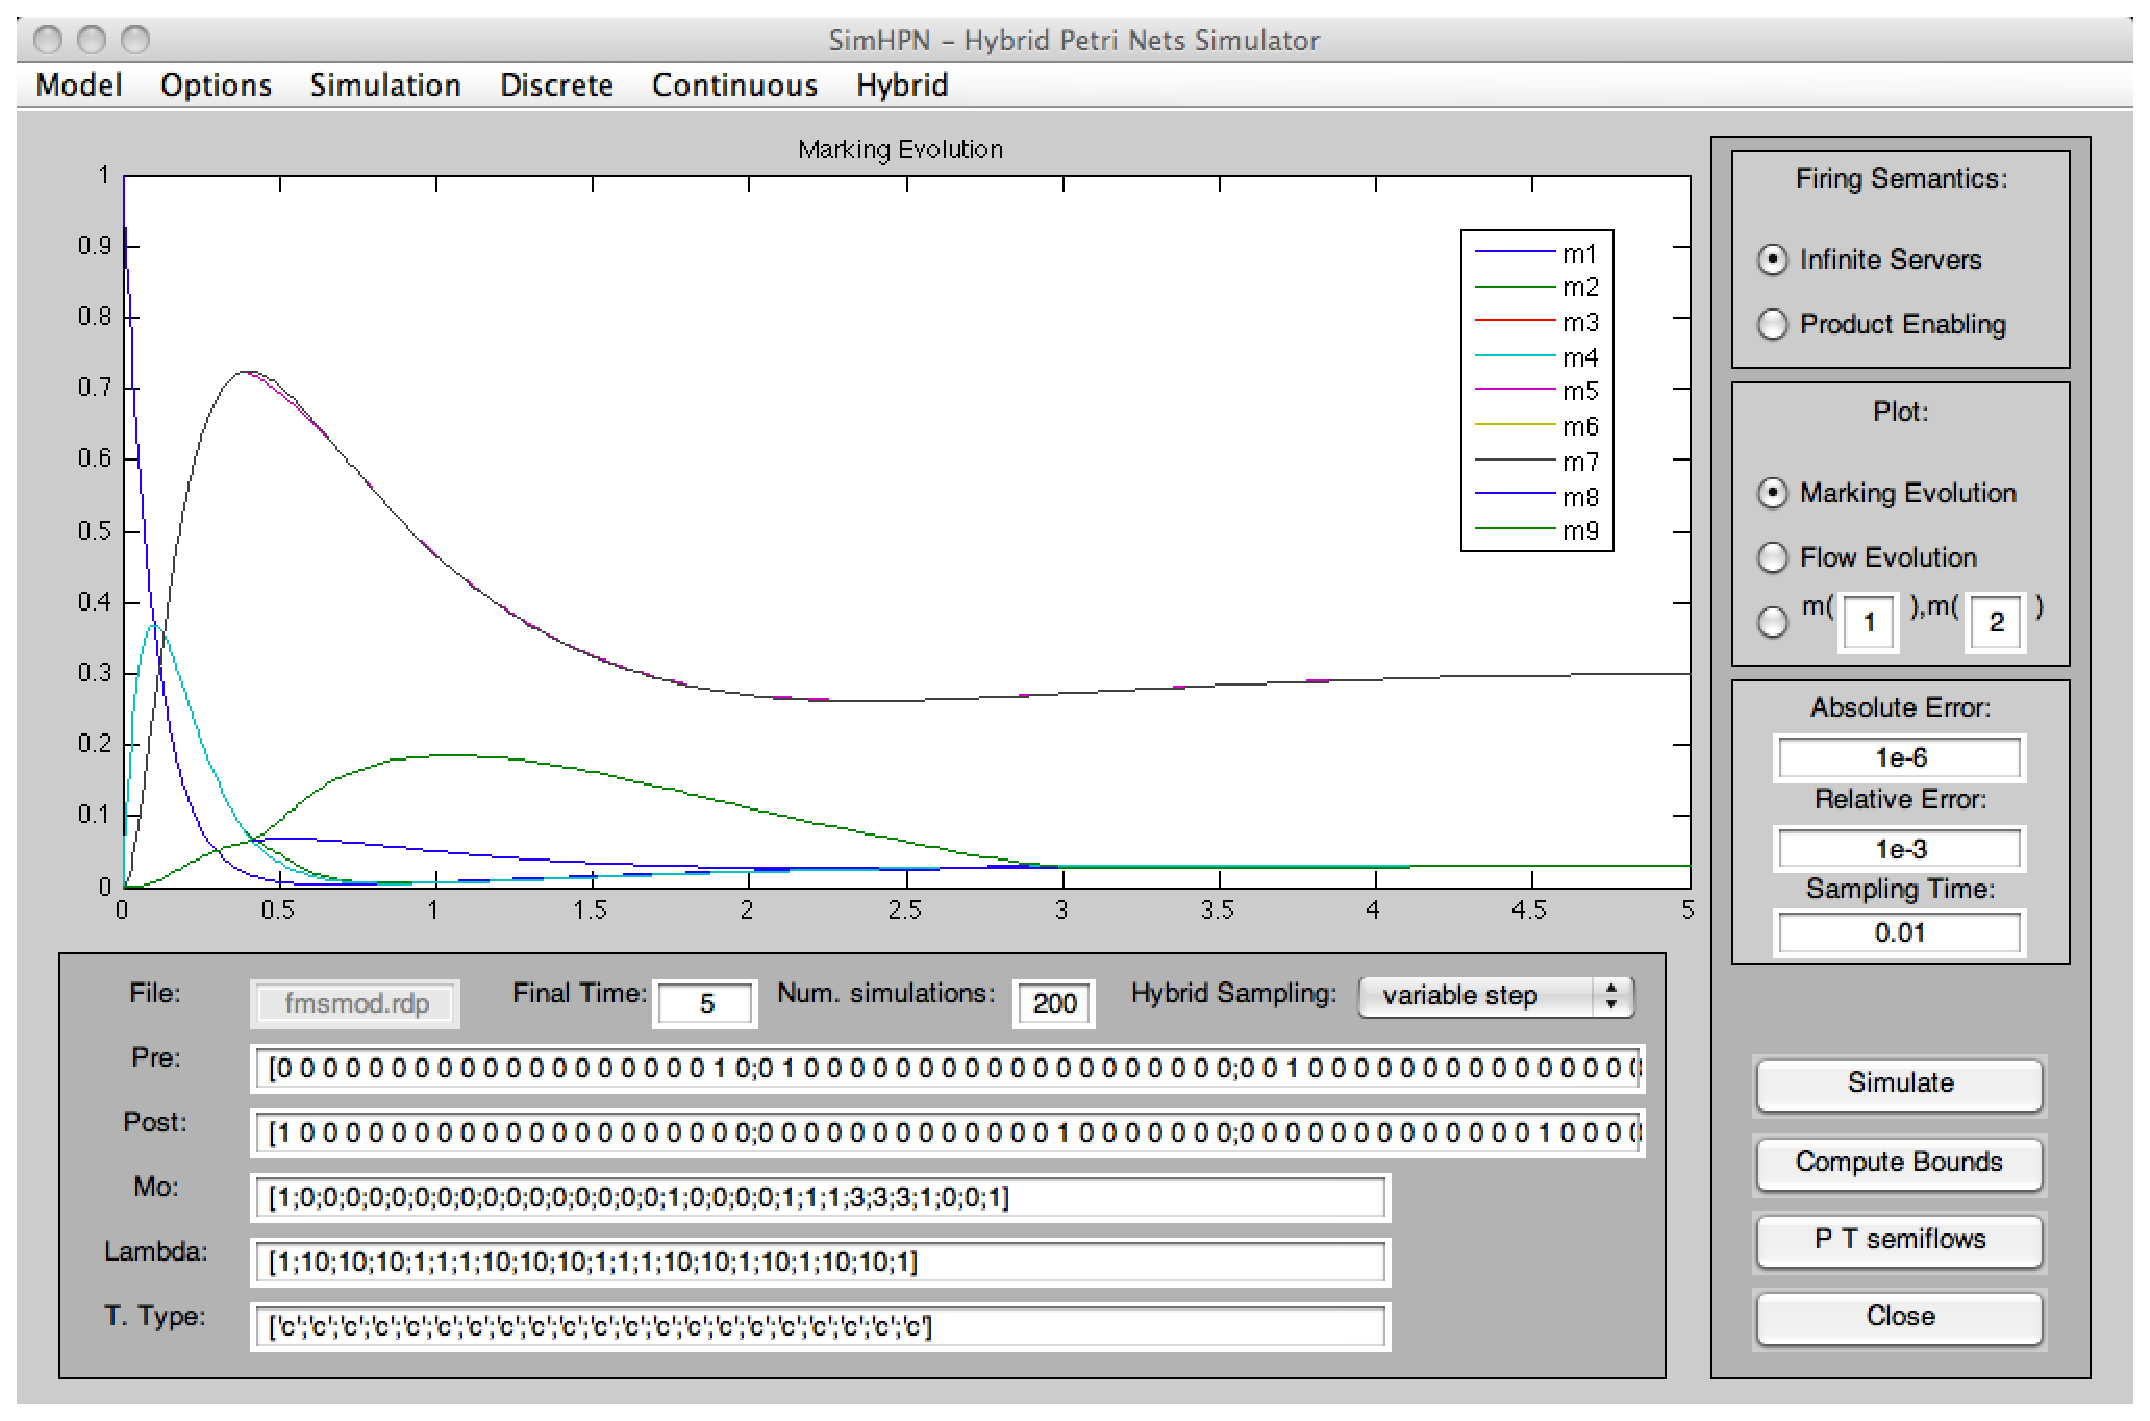
\includegraphics[width=1\columnwidth]{figs/mainScreen.eps}}
   \caption{Sketch of the main window of SimHPN}
   \label{f-main}
\end{figure}


\newpage

\input{Installation}


\chapter{Petri nets overview}
%\addcontentsline{toc}{chapter}{Brief introduction to contPN}
%\markboth{Brief introduction to contPN}{Brief introduction to contPN}

Hybrid Petri nets~\cite{BODavid10,ARBaMeGi00} represent a powerful modeling formalism
that allows the integration of both continuous and discrete dynamics in a single net model. This
section defines the class of hybrid nets supported by $SimHPN$. In the following, the reader
is assumed to be familiar with Petri nets (PNs) (see \cite{ARMura89,BODHPSV93}
for a gentle introduction).

\section{Untimed Hybrid Petri net  systems}
\label{s:untimedHPN}

\begin{defn}
\label{d:uhpn}
A \emph{Hybrid Petri Net (HPN) system} is a pair $\sys$, where: $\N = \langle
P,T,\Pre,\Post\rangle$ is a \emph{net structure}, with set of places
$P$, set of transitions $T$, pre and post incidence matrices
$\Pre, \Post \in \rea^{|P|\times |T|}_{\geq 0}$, and $\b{m}_0\in \rea^{|P|}_{\geq 0}$ is the
\emph{initial marking}.
\end{defn}

% Definition of structural elements
The token load of the place $p_i$ at marking $\b{m}$ is denoted by
$m_i$ and the \emph{preset} and \emph{postset} of a node $X \in P \cup
T$ are denoted by $\preset{X}$ and $\postset{X}$, respectively. For
a given incidence matrix, e.g., $\Pre$, $\Pre(p_i,t_j)$ denotes the element of
$\Pre$ in row $i$ and column $j$.

\begin{figure*}
\centering
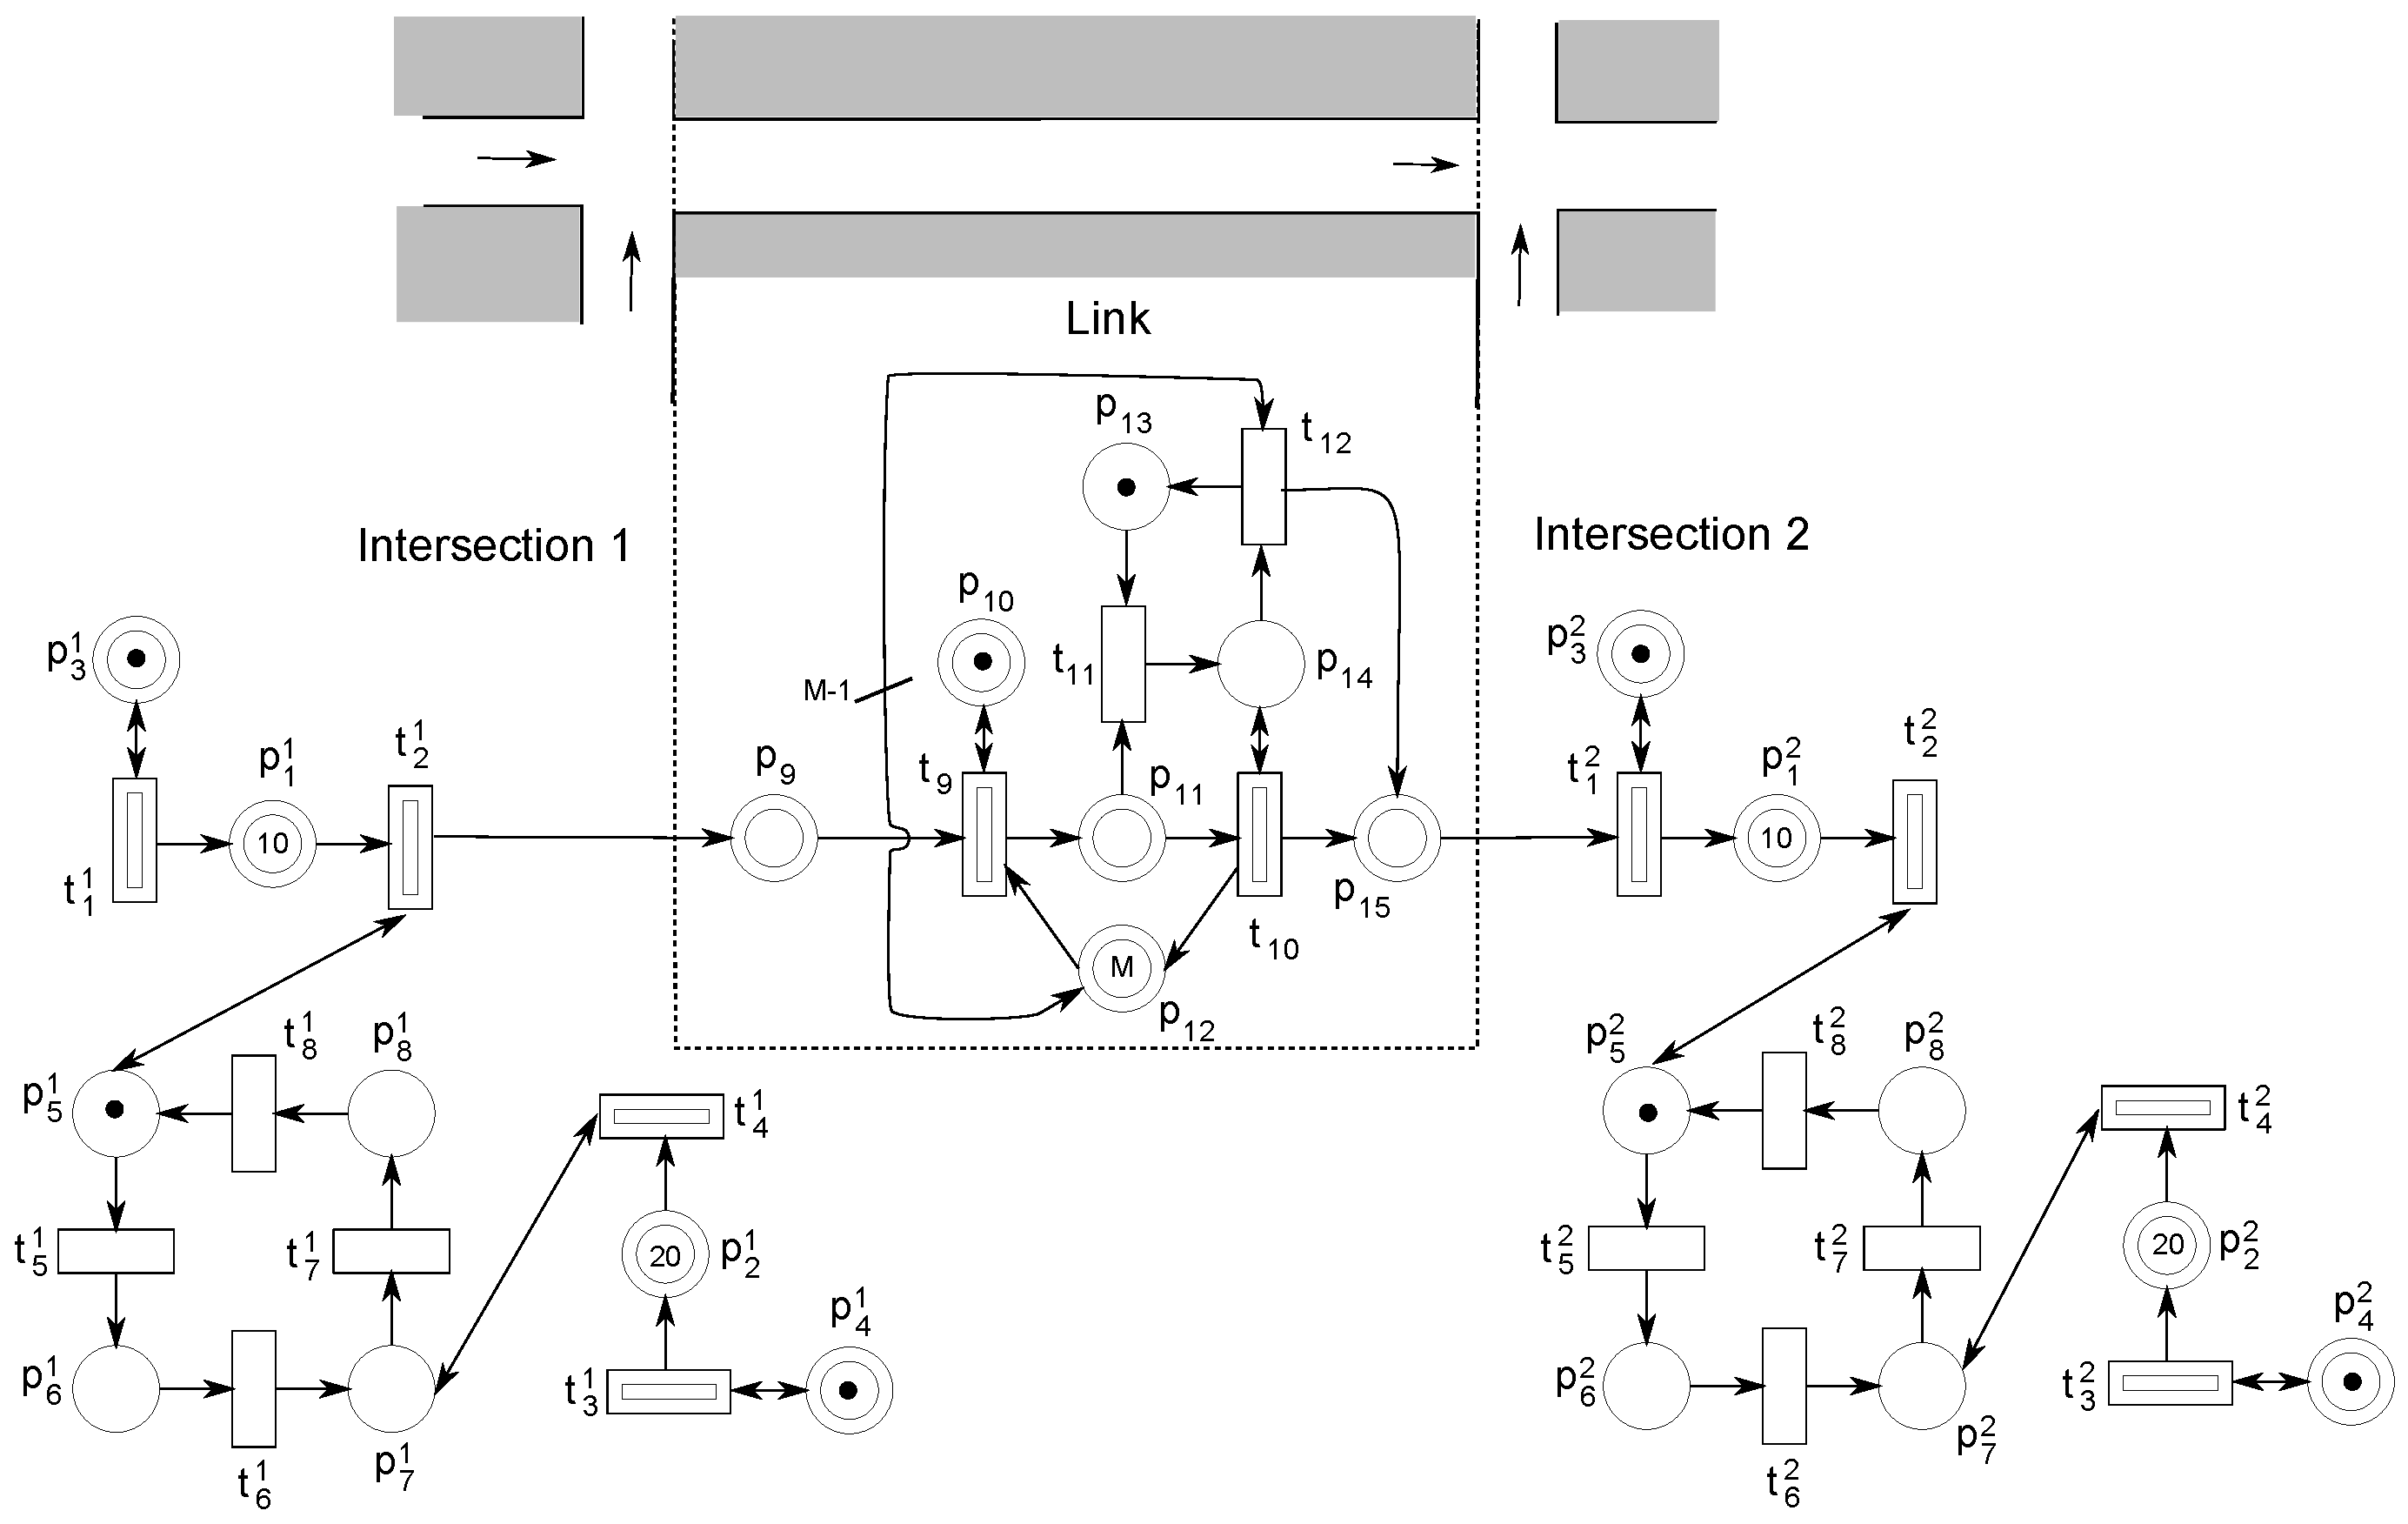
\includegraphics[width=.81\textwidth]{figs/modelo2}
\caption{$HPN$ model of $2$ intersections connected by a link.}
\label{f-traffic}
\end{figure*}


In a HPN, the set of transitions $T$ is partitioned in two sets $T=T^c\cup T^d$,
where $T^c$ contains the set of continuous transitions and $T^d$ the set of discrete
transitions. In contrast to other works, the set of places $P$ is not explicitly
partitioned, i.e., the marking of a place is a natural or real number depending on the
firings of its input and output transitions. Nevertheless, in order to make net models
easier to understand, those places whose marking can be a real non-integer number
will be depicted as double circles (see $p_1^1$ in Fig.~\ref{f-traffic}), and the rest of places will be
depicted as simple circles (such places will have integer markings, see $p_5^1$ in Fig.~\ref{f-traffic}).
Continuous transitions are graphically depicted as two bars (see $t_4^1$ in Fig.~\ref{f-traffic}), while
discrete transitions are represented as empty bars (see $t_5^1$ in Fig.~\ref{f-traffic}), .

Two enabled transitions $t_i$ and $t_j$ are in conflict when they cannot
occur at the same time. For this, it is necessary that $\preset{t_i} \,
\cap \preset{t_j} \neq \emptyset$, and in that case it is said that
$t_i$ and $t_j$ are in structural conflict relation.
%When $\Pre[P,t_i]=\Pre[P,t_j] \neq \zeros$, $t_i$ and $t_j$ are said to be in \emph{equal conflict} relation.
Right and left non negative annullers of the token flow matrix
$\b{C}$ are called T- and P-\emph{semiflows}, respectively.
A semiflow $\vect{v}$ is \emph{minimal} when its
support, $\support{\vect{v}}=\{i\spbar \vect{v}(i)\neq 0\}$, is
not a proper superset of the support of any other semiflow, and
the greatest common divisor of its elements is one.
If there exists $\b{y}>0$ such that $\b{y} \cdot \b{C}=0$,  the net is said to be
\emph{conservative}, and if there exists $\b{x}>0$ satisfying $\b{C}\cdot\b{x}=0$,  the net
is said to be \emph{consistent}. As it will be seen, the basic tasks that
$SimHPN$ can perform on untimed hybrid Petri nets are related to the
computation of minimal T- and P-semiflows.

% Enabling and firing rule
The enabling degree of a continuous transition $t_j \in T$ is:
\begin{equation}
\label{eq:enab}
enab(t_j,\b{m}) = \begin{cases}
 \min \limits_{p_i \in \preset{t_j}}  \left\lfloor\dfrac{m_i}{\Pre(p_i,t_j)}\right\rfloor & \text{ if $t_j \in T^d$}
  \vspace{.2cm}
\\
 \min \limits_{p_i \in \preset{t_j}} \dfrac{m_i}{\Pre(p_i,t_j)} & \text{ if $t_j \in T^c$}
\end{cases}
\end{equation}

Transition $t_j \in T$ is \emph{enabled} at $\b{m}$ iff $enab(t_j,\b{m})>0$.
An enabled transition $t_j \in T$ can fire in any amount $\alpha$ such that
\mbox{$0 \leq \alpha \leq enab(t_j,\b{m})$} and $\alpha\in\nat$ if $t_j \in T^d$
and \mbox{$\alpha\in\rea$} if $t_j \in T^c$. Such a firing leads to a
new marking \mbox{$\b{m'} = \b{m} + \alpha \cdot \C(\cdot,t_j)$}, where $\C = \Post
- \Pre$ is the token-flow matrix and $\C(\cdot,t_j)$ is its $j$ column. If $\b{m}$ is reachable from
$\b{m}_0$ through a finite sequence $\sigma$, the \emph{state (or
fundamental) equation}, $\b{m} =\b{m}_0
+\C \cdot \b{\sigma}$ is satisfied, where $\b{\sigma} \in \rea^{|\mathit{T}|}_{\geq 0}$
is the firing count vector. According to this firing rule the class of nets defined
in Def~\ref{d:uhpn} is equivalent to the class of nets defined in~\cite{BODavid10,ARBaMeGi00}.


\section{Timed Hybrid Petri net  systems}
\label{s:timedHPN}

Different time interpretations can be associated to the firing of transitions.
Once an interpretation is chosen, the state equation can be used to show
the dependency of the marking on time, i.e., $\b{m}(\tau) = \b{m_0} + \C \cdot
\b{\sigma}(\tau)$. The term $\b{\sigma}(\tau)$ is the firing count vector
at time $\tau$. Depending on the chosen time interpretation, the firing
count vector $\sigma_j(\tau)$ of a transition $t_j \in T^c$ is differentiable
with respect to time, and its derivative $f_j(\tau)=\dot{\sigma_j}(\tau)$
represents the \emph{continuous flow} of $t_j$. As for the timing of
discrete transitions, several definitions exist for the flow of continuous
transitions. $SimHPN$ accounts for infinite server and product server semantics
in both continuous and discrete transitions, and additionally, discrete transitions
are also allow to have deterministic delays.

\begin{defn}
\label{d:thpn}
A \emph{Timed Hybrid Petri Net (THPN) system} is a tuple $\langle \N, \b{m}_0, Type, \b{\lambda} \rangle$
where $\langle \N, \b{m}_0\rangle$ is a HPN, $Type:T\rightarrow \{id,pd,dd,ic,pc\}$ establishes the time
semantics of transitions and $\b{\lambda}:T\rightarrow \rea_{\geq 0}$ associates a real parameter to each
transition related to its semantics.
\end{defn}

Any of the following semantics is allowed for a discrete transition $t_i\in T^d$:
\begin{itemize}
\item \emph{Infinite server semantics} ($Type(t_i)=id$): Under infinite server
semantics, the time delay of a transition $t_i$, at a given marking $\b{m}$, is an exponentially distributed
random variable with parameter $\lambda_i\cdot enab(t_i,\b{m})$,
where the integer enabling $enab(t_i,\b{m})$ represents the number of active servers of
$t_i$ at marking $\b{m}$.
\item \emph{Product server semantics} ($Type(t_i)=pd$): Under product server
semantics, the time delay of a transition $t_i$ at $\b{m}$ is an exponentially
distributed random variable with parameter $\lambda_i \cdot
\prod\limits_{p_j\in \preset{t_i}} \left\lfloor\dfrac{\b{m}(p_j)}{\b{Pre}(p_j,t_i)}\right\rfloor$, where
$\prod\limits_{p_j\in \preset{t_i}} \left\lfloor\dfrac{\b{m}(p_j)}{\b{Pre}(p_j,t_i)}\right\rfloor$ is the number of active servers.
\item \emph{Deterministic delay} ($Type(t_i)=dd$): A transition $t_i$ with deterministic
delay is scheduled to fire $1/\lambda_i$ time units after it became enabled.
\end{itemize}

\emph{Conflict resolution:} When several discrete exponential transitions, under either infinite or product server semantics, are in conflict, a racing policy is adopted, i.e., the one with smaller time delay will fire first.

If a discrete transition with deterministic delay is not in conflict with other transitions, it is fired as scheduled, if it is in conflict then
it is fired only if its schedule firing time is less than the firing time of the conflicting
transition. The transition to fire, in the case of several conflicting deterministic transitions
with same scheduled firing instance, is chosen probabilistically assigning the same probability
to each conflicting transition. Furthermore after the firing of a
deterministic transition, the timers of all the transitions in the same conflict are discarded.

For a continuous transition $t_i\in T^c$ the following semantics are allowed:
\begin{itemize}
\item \emph{Infinite server semantics} ($Type(t_i)=ic$): Under \emph{infinite server}
the flow of a transition $t_i$ is:
\begin{equation}\label{eq-flowinf}
f_i=\lambda_i \cdot enab(t_i,\b{m}) = \lambda_i \cdot \min
\limits_{p_j \in \preset{t_i}} \left\{ \frac{m_j}{\b{Pre}(p_j,t_i)}
\right\}
\end{equation}
Such an expression for the flow is obtained from a first order approximation of the
discrete case~\cite{ARSiRe02} and corresponds to the \emph{variable speed} of
(\cite{ARAlDa98})
\item \emph{Product server  semantics} ($Type(t_i)=pc$): In a similar way to discrete
transitions, the continuous flow under product server semantics is given by:
$$f_i=\lambda_i\cdot\prod_{p_j\ \in\ \preset{t_i}}{\biggl\{\frac{m_j}{\b{Pre}(p_j,t_i)}\biggr\}}$$
\end{itemize}

The described supported semantics cover the modeling of a large variety of actions
usually associated to transitions. For instance, infinite server semantics, which are
more general than finite server semantics, are well suited for modeling actions in
manufacturing, transportation and logistic systems~\cite{BODavid10}; product server semantics are
specially useful to modeling population dynamics~\cite{IPSiRe00} and biochemical
reactions~\cite{InHeGiDo08}; and deterministic delays allow one to represent pure
delays and clocks that appear, for instance, when modeling traffic lights in
automotive traffic systems~\cite{IPVaSuBoSi10}.

\newpage



\chapter{Using SimHPN}

\section{Short description of the GUI}
The $SimHPN$ simulator supports {\color{red} infinite server} and {\color{red}product server semantics} for both discrete and continuous transitions. Moreover, deterministic delays with single server semantics are also supported for discrete transitions. Both the data related to the model description, i.e., net structure, initial marking and timing parameter, and the output results, i.e., time trajectories, are MATLAB variables. At the end of the simulation, the user can export the data to the MATLAB workspace where can be used for further analysis. 

The $SimHPN$ toolbox (\url{http://webdiis.unizar.es/GISED/?q=tool/simhpn}) provides a Graphical User Interface (GUI) that enables the user to easily perform simulations and carry out analysis methods.  This GUI consists of a MATLAB figure window, exhibiting a \emph{Menu bar} and three control panels: 
\begin{itemize}
\item[(i)] \emph{Drawing Area}, 
\item[(ii)] \emph{Options panel}, and 
\item[(iii)] \emph{Model Management panel}. 
\end{itemize}
Fig. \ref{GUI} presents a hard-copy screenshot of the main window opened by $SimHPN$ toolbox, where all the component parts of the GUI are visible.

\begin{figure*}[!htb]
   \centering{
   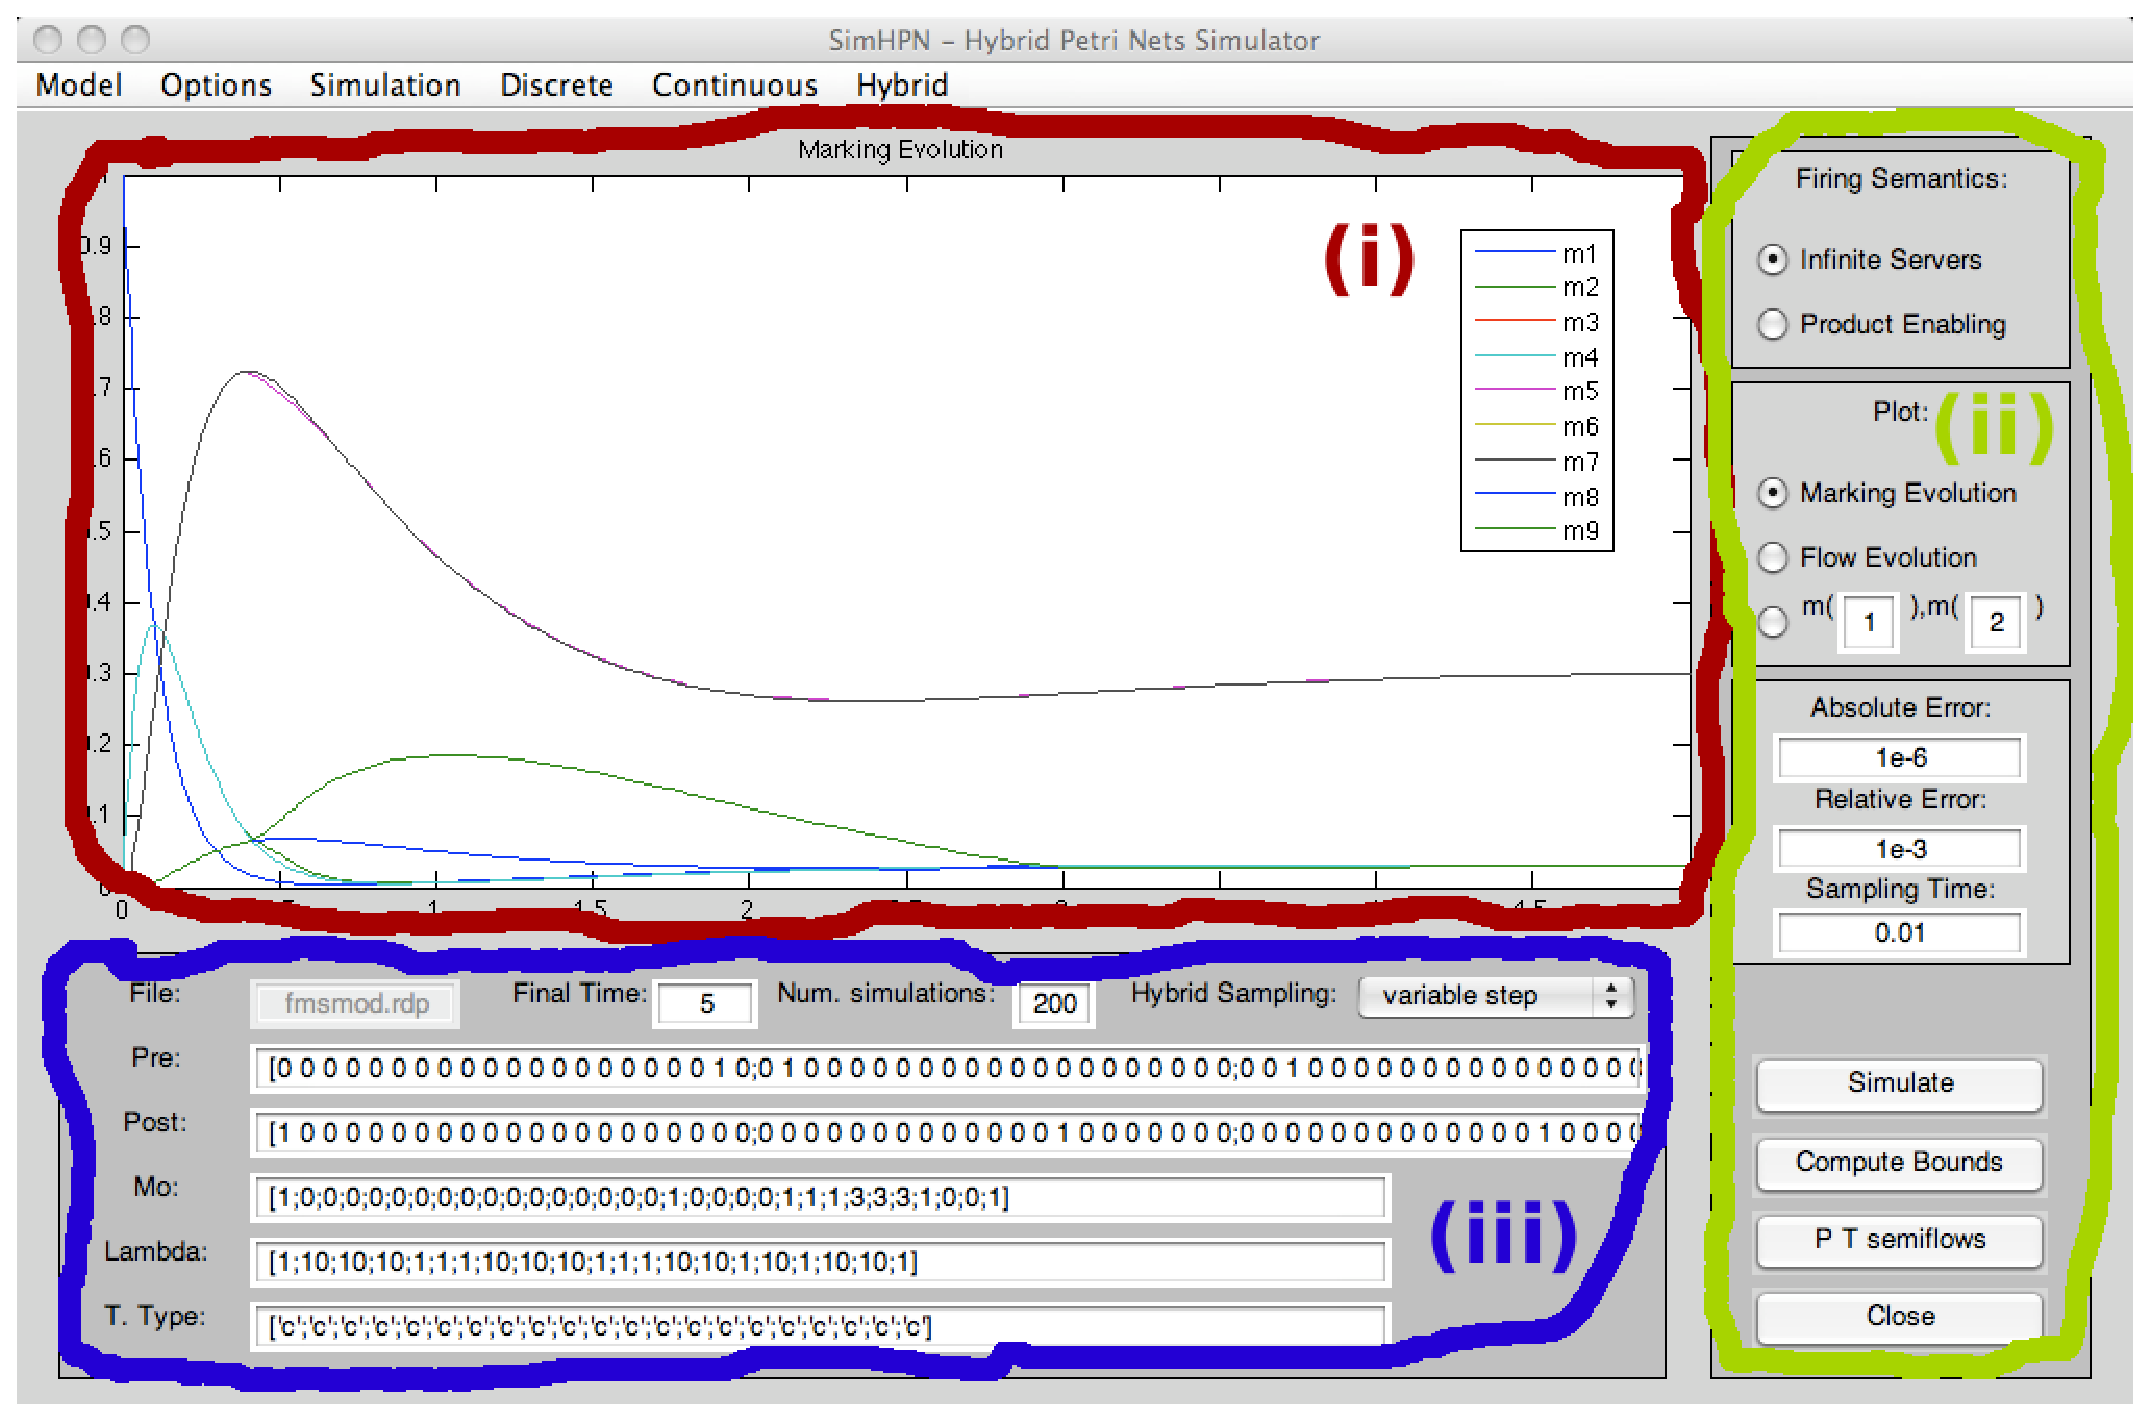
\includegraphics[width=.85\textwidth]{figs/mainScreen2.eps}}
   \caption[htb!]{Sketch of the main window of $SimHPN$}\label{GUI}
\end{figure*}

The \emph{Menu bar} (placed horizontally, on the top of the window in Fig. \ref{GUI}) displays a set of six drop-down menus at the top of the window, where the user can select different features available in the $SimHPN$ toolbox. These menus are: \emph{Model}, \emph{Options}, \emph{Simulation}, \emph{Discrete}, \emph{Continuous} and \emph{Hybrid}.

The {\color{blue}\emph{Model menu}} contains the pop-up menus:
\begin{itemize}
\item \emph{Import from Pmeditor}, 
\item \emph{Import from TimeNet} and 
\item \emph{Import from .mat file} 
\item \emph{Save to .mat file}
\end{itemize}
that implement several importing options for the matrices, $\b{Pre}$, $\b{Post}$, $\mo$, etc, that describe the net system. Such matrices can be introduced manually or through two Petri nets editors: PMEditeur and TimeNet \cite{IPZiKn95}.  Moreover, the matrices can be automatically loaded from a $.mat$ file (MATLAB file format) or loaded from variables defined in the workspace, this is done just by writing the name of the variable to be used in the corresponding edit boxes. 

If the model is imported from a $.mat$ file, the following variables should be defined in the $.mat$ file:

\begin{itemize}
\item $Pre$ - is a $|P| \times$ $|T|$ matrix containing the weight of the arcs from places to transitions;
\item $Post$ - is a $|P| \times$ $|T|$   containing the weight of the arcs from transitions to places;
\item $M0$ - is a column vector of dimension $|P|$ containing the initial marking;
\item $Lambda$ - is a column vector of dimension $|T|$ containing the firing rates of transitions:
\item $Trans\_Type$ - is a column vector of dimension $|T|$ containing the type of transitions. Each element can have one of the following values:
\begin{itemize}
\item $'c'$ - for continuous transition;
\item $'d'$ - for stochastic discrete transitions;
\item $'q'$ -  for deterministic  discrete transitions.
\end{itemize}
\end{itemize}


The last option (i.e., \emph{Save to .mat file}) saves to a .mat file the matrices already defined in the edit boxes of $SimHPN$.

The {\color{blue}\emph{Options}} menu contains only the pop-up menu 
\begin{itemize}
\item \emph{Show Figure Toolbar} 
\end{itemize}
that allows to show the characteristic toolbar of the MATAB figure object that permits, for example, the use of zoom tool on the displayed graphic in the \emph{Drawing Area}.

The {\color{blue}\emph{Simulation menu}} contains the pop-up menus: 
\begin{itemize}
\item \emph{Markings to plot}, 
\item \emph{Flows to plot}, and 
\item \emph{Save results to workspace}. 
\end{itemize}
The pop-up menus \emph{Markings to plot}, \emph{Flows to plot} allow the user to select the components of marking vector and flow vector that will be plotted after  simulation in the \emph{Drawing area}. The pop-up menu \emph{Save results to workspace}  permits to export, after simulation, the marking and flow evolution to variables in the MATLAB workspace.

The following the menus call procedure for analysis and synthesis of PN model if it is assumed discrete Petri net (\emph{Discrete} menu), fully continuous Petri net (\emph{Continuous} menu) and Hybrid Petri net (\emph{Hybrid} menu).

The {\color{blue}\emph{Continuous menu}} contains the pop-up menus:
\begin{itemize}
\item \emph{Control}
\item \emph{Optimal}
\item \emph{Diagnosis}
\end{itemize} 

The Control submenu contains the pop-up menus \emph{Control law} and \emph{Save results to workspace} that permit the designing of a control law to reach a desired final marking if the net is continuous under infinite server semantics. 

The \emph{Optimal} submenu contains the pop-up menus \emph{Optimal Observability} and \emph{Optimal Control}. Such pop-up menus perform calls to the algorithms for computing optimal steady state and optimal sensor placement for continuous Petri nets with infinite server semantics.

The \emph{Diagnosis} submenu calls the algorithms that perform fault diagnosis for untimed continuous Petri nets \cite{ARMASECASI12}. Once the user selects this option, a window as in Fig.~\ref{fig:diag} is opened and the user should introduce the input parameters:
\begin{enumerate}
\item The number of observable transitions. Without loss of generality, it is assumed that the first transitions are observable and the rest are unobservable.
\item The firing sequence of observable transitions.
\item The firing amount of each transition of the firing sequence.
\item Number of fault classes.
\end{enumerate}


\begin{figure*}[!htb]
   \centering{
   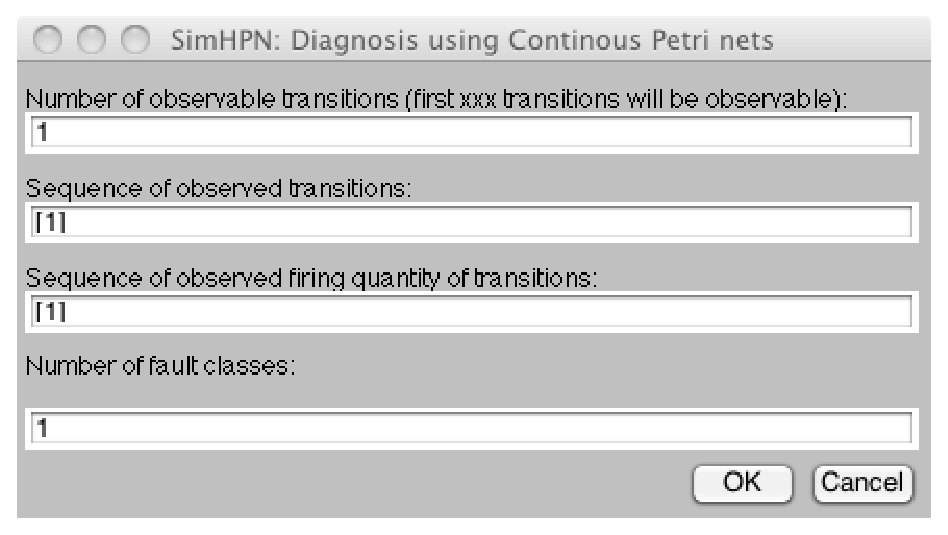
\includegraphics[width=.85\textwidth]{figs/diag1.eps}}
   \caption[htb!]{Sketch of the uicontrols for the diagnosis.}\label{fig:diag}
\end{figure*}

After this, an uicontrol will be used to introduce the transitions belonging to each fault class. All the results are shown at the MATLAB command prompt. See Section~\ref{sec:fdsexamps} for examples and more details on the parameters for fault detection.


The \emph{Drawing area} (located in the left and central side of the window in Fig. \ref{GUI}), is a MATLAB axes object where the trajectories of the simulation results are plotted. The components of markings and flows that will be represented are selected from the menu.

The \emph{Options panel} (placed, as a horizontal bar, on the right part of the window Fig. \ref{GUI}) presents a number of options related to the model. From top to bottom: (a) two radio buttons to select the firing semantics for continuous and discrete exponential  transitions; (b) three radio buttons allowing to select the variables to be plotted in the \emph{Drawing Area}, the simulator allows one to plot the evolution of the marking
of the places, the evolution of the flow of the transitions and
the evolution of the marking of one place vs. the marking of other
place; (c) three edit boxes to fix the maximum absolute and relative errors allowed by the simulated trajectory and the sampling time used in simulations (see next subsection for more details on the selection of the sampling time); (d) a \emph{Simulate} button to start a new simulation; (e) a \emph{Compute Bounds} button that computes performance bounds for continuous nets under infinite server semantics; (f) a \emph{P T semiflows} button to compute the minimal P- and T-semiflows of the net, the results are displayed on the MATLAB command window and can be used for future analysis tasks; and (g) a \emph{Close} button to close the $SimHPN$ toolbox.

The \emph{Model Management Panel} panel is composed of different edit boxes (placed in the bottom left corner of the window in Fig. \ref{GUI}), where the $SimHPN$ toolbox displays the current values of the matrices describing the net system and permits to select the simulation time and the number of simulations to be performed (this last parameter is ignored if the net contains no stochastic transitions).  The required matrices for a system in order to be simulated are: $\b{Pre}$ and $\b{Post}$ matrices, initial marking $\mo$, the parameter $\b{\lambda}$ of each transition, and the type of each transition. This last parameter is equal to 'c' for continuous transitions, to 'd' for stochastic discrete transitions and to 'q' for deterministic discrete transitions. Notice that if the type of a transition is 'q' then single server semantics is adopted for its firing and therefore the selection of firing semantics in the \emph{Options panel} will be ignored for this transition.

\section{Script simulation}
$SimHPN$ permits the simulation of a hybrid Petri net from the MATLAB prompt, without open the GUI. This is useful if one wants to implement a script and simulate a hybrid Petri net for some particular input parameters. This can be done in two different ways depending on the type of the input model.

\textbf{Continuous Petri net}. If the net has only continuous transitions, the following command can be used for its simulation:

\begin{verbatim}
[m,f,t] = SimHPN_Simul(Pre, Post, m0, tf, lambda, seman, erel, eabs);
\end{verbatim}
where, 
\begin{itemize}
\item $Pre$ - is a $|P| \times$ $|T|$ matrix containing the weight of the arcs from places to transitions;
\item $Post$ - is a $|P| \times$ $|T|$   containing the weight of the arcs from transitions to places;
\item $m0$ - is a column vector of dimension $|P|$ containing the initial marking;
\item $tf$ - is the final time for simulation;
\item $lambda$ - is a column vector of dimension $|T|$ containing the firing rates of transitions:
\item $seman = 1$ - if transitions are with infinite server semantics and $seman = 2$ - if product firing semantics is considered for transitions;
\item $erel$ - relative error;
\item $eabs$ - absolute error.
\end{itemize}

The returned parameters are:

\begin{itemize}
\item $m$ - a matrix of dimension $|t| \times |P|$ is the matrix defining the marking evolutions;
\item $f$ - a matrix of dimension $|t| \times |T|$ is the matrix defining the flow evolutions;
\item $t$ - a row vector containing the time instants for which the markings and the flows are defined.
\end{itemize}

\textbf{Hybrid Petri net}. If the net is not purely continuous, function \emph{SimHPN\_SimHyb} 
should be used. This function is defined as follows:

\begin{verbatim}
[m,f,t] = SimHPN_SimHyb(Pre,Post,lambda,type,m0,nsim,tsim,seman,mode,delta)
\end{verbatim}

The input parameters are:

\begin{itemize}
\item $Pre$ - is a $|P| \times$ $|T|$ matrix containing the weight of the arcs from places to transitions;
\item $Post$ - is a $|P| \times$ $|T|$   containing the weight of the arcs from transitions to places;
\item $lambda$ - is a column vector of dimension $|T|$ containing the firing rates of transitions:
\item $type$ - is a column vector of dimension $|T|$ containing the type of transitions. Each element can have one of the following values:
\begin{itemize}
\item $'c'$ - for continuous transition;
\item $'d'$ - for stochastic discrete transitions;
\item $'q'$ -  for deterministic  discrete transitions.
\end{itemize}
\item $m0$ - is a column vector of dimension $|P|$ containing the initial marking;
\item $nsim$ - number of simulations especially useful for stochastic transitions;
\item $tsim$ - simulation time
\item $seman = 1$ - if continuous transitions are with infinite server semantics and $seman = 2$ is product firing semantics is considered for continuous transitions;
\item $mode = 1$ - if constant hybrid sampling step will be used;  $mode = 2$ - if variable hybrid sampling step will be used;  
\item $delta$ - sampling timed used in the case of $mode = 1$.
\end{itemize}
 
 After a simulation, the returned parameters are:

\begin{itemize} 
\item $m$ - a matrix of dimension $|t| \times |P|$ is the matrix defining the marking evolutions;
\item $f$ - a matrix of dimension $|t| \times |T|$ is the matrix defining the flow evolutions;
\item $t$ - a row vector containing the time instants for which the markings and the flows are defined.
\end{itemize}

\newpage



\chapter{Examples of utilization}

This section presents some systems that are analyzed and simulated using $SimHPN$.

\section{An assembly line}
\label{s:assembly}

The Petri net system in Fig.~\ref{cas:f-fmsmod} represents an
assembly line with kanban strategy (see~\cite{ZRS-JIM-01}). The
system has two stages that are connected by transition $t_{14}$.
The first stage is composed of three lines (starting from $p_2$,
$p_3$ and $p_4$ respectively) and three machines ($p_{23}$,
$p_{24}$ and $p_{25}$). Places $p_{26}$, $p_{27}$ and $p_{28}$ are
buffers at the end of the lines. The second stage has two lines
that require the same machine/resource $p_{18}$. The number of
kanban cards is given by the marking of places $p_2$, $p_3$ and
$p_4$ for the first stage, and by the marking of $p_{32}$ for the
second stage. The system demand is given by the marking of $p_1$.
We will make use of this net system to illustrate some of the
features of $SimHPN$.

\begin{figure*}[!hbt]
\psfrag{t1}{$t_1$}\psfrag{t2}{$t_2$}\psfrag{t3}{$t_3$}\psfrag{t4}{$t_4$}\psfrag{t5}{$t_5$}\psfrag{t6}{$t_6$}
\psfrag{t7}{$t_7$}\psfrag{t8}{$t_8$}\psfrag{t9}{$t_9$}\psfrag{t10}{$t_{10}$}\psfrag{t11}{$t_{11}$}\psfrag{t12}{$t_{12}$}
\psfrag{t13}{$t_{13}$}\psfrag{t14}{$t_{14}$}\psfrag{t15}{$t_{15}$}\psfrag{t16}{$t_{16}$}\psfrag{t17}{$t_{17}$}\psfrag{t18}{$t_{18}$}
\psfrag{t19}{$t_{19}$}\psfrag{t20}{$t_{20}$}\psfrag{t21}{$t_{21}$}
\psfrag{p1}{$p_1$}\psfrag{p2}{$p_2$}\psfrag{p3}{$p_3$}\psfrag{p4}{$p_4$}\psfrag{p5}{$p_5$}\psfrag{p6}{$p_6$}\psfrag{p7}{$p_7$}
\psfrag{p8}{$p_8$}\psfrag{p9}{$p_9$}\psfrag{p10}{$p_{10}$}\psfrag{p11}{$p_{11}$}\psfrag{p12}{$p_{12}$}\psfrag{p13}{$p_{13}$}\psfrag{p14}{$p_{14}$}
\psfrag{p15}{$p_{15}$}\psfrag{p16}{$p_{16}$}\psfrag{p17}{$p_{17}$}\psfrag{p18}{$p_{18}$}\psfrag{p19}{$p_{19}$}\psfrag{p20}{$p_{20}$}\psfrag{p21}{$p_{21}$}
\psfrag{p22}{$p_{22}$}\psfrag{p23}{$p_{23}$}\psfrag{p24}{$p_{24}$}\psfrag{p25}{$p_{25}$}\psfrag{p26}{$p_{26}$}\psfrag{p27}{$p_{27}$}\psfrag{p28}{$p_{28}$}
\psfrag{p29}{$p_{29}$}\psfrag{p30}{$p_{30}$}\psfrag{p31}{$p_{31}$}\psfrag{p32}{$p_{32}$}
    \centering{
         {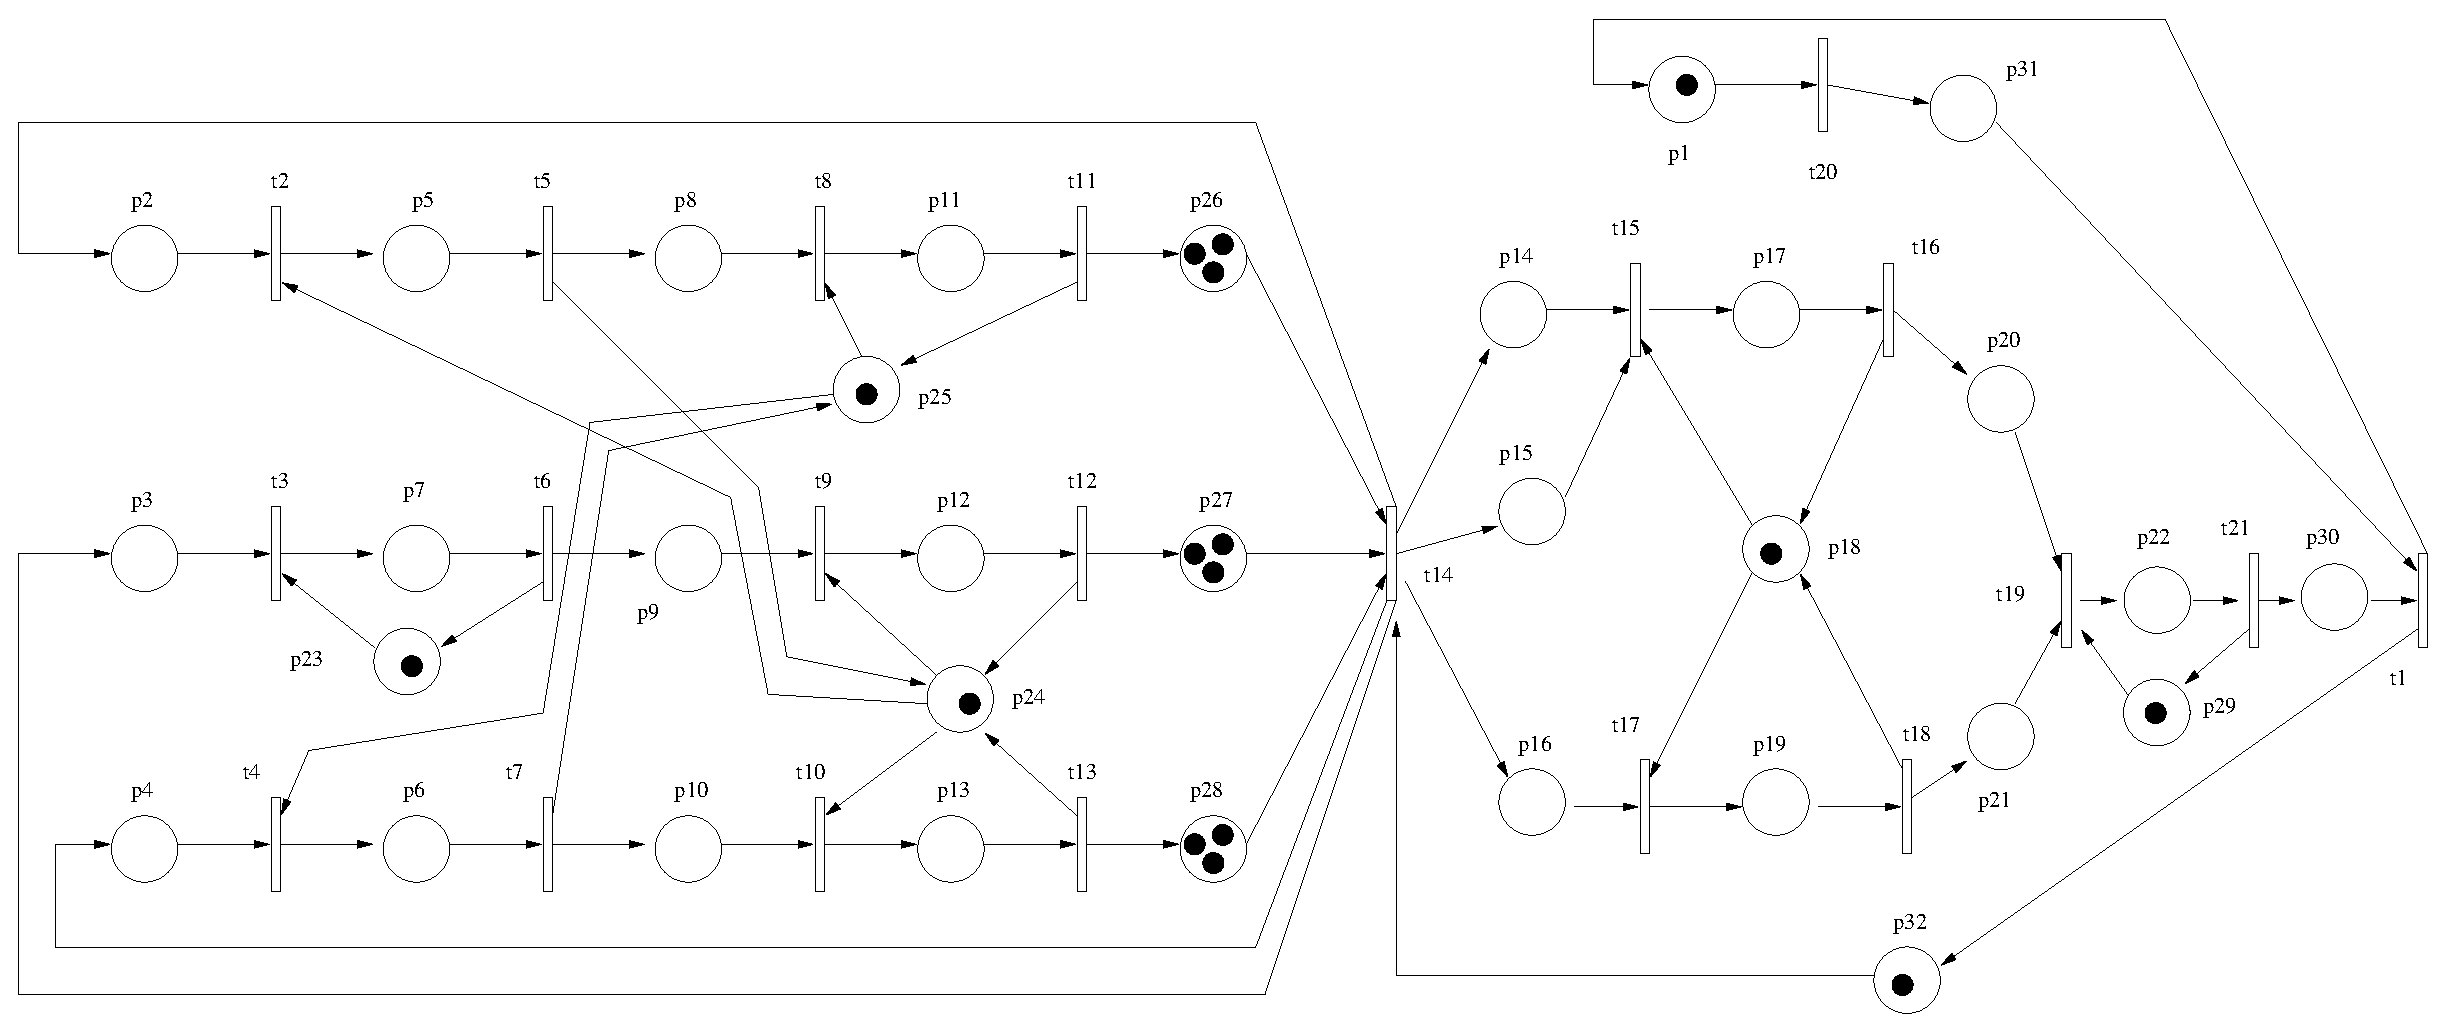
\includegraphics[width=0.95\linewidth] {figs/fmsmodi.eps}}
       }
    \caption[]{An assembly line with kanban strategy.}
   \label{cas:f-fmsmod}
\end{figure*}

Given that all transitions represent actions that can potentially have
high working loads, all transitions are considered continuous.
Moreover, infinite server semantics will be adopted for all of them. Let
the initial marking be $\mo(p_1)=\mo(p_{18})=\mo(p_{23})=\mo(p_{24})=\mo(p_{25})=\mo(p_{29})=\mo(p_{32})=1$,
$\mo(p_{26})=\mo(p_{27})=\mo(p_{28})=3$ and the marking of the
rest of places be equal to zero. Let us assume that the firing rates of the transitions are
$\la(t_2)=\la(t_3)=\la(t_4)=\la(t_8)=\la(t_9)=\la(t_{10})=\la(t_{14})=\la(t_{15})=\la(t_{17})=\la(t_{19})=\la(t_{20})=10$,
$\la(t_1)=\la(t_5)=\la(t_6)=\la(t_7)=\la(t_{11})=\la(t_{12})=\la(t_{13})=\la(t_{16})=\la(t_{18})=\la(t_{21})=1$.

{\bf Computation of minimal P-T \emph{semiflows}:} $SimHPN$ implements
the algorithm proposed in~\cite{BOSilv85} to compute the minimal P-\emph{semiflows} of a Petri net. The same algorithm applied on the transpose of the incidence matrix yields the minimal T-\emph{semiflows} of the net. Notice that P and T-\emph{semiflows}
just depend on the structure of the net and not on the continuous or discrete
nature of the transitions. The result of applying the algorithm on the net
in Fig.~\ref{cas:f-fmsmod} is the set of  $12$ minimal P-semiflows that
cover every place, i.e., it is conservative, and the set that contains the only
minimal T-semiflow  which is a vector of ones, i.e., it is consistent.


{\bf Throughput bounds:}  When all transitions are continuous and work
under infinite server semantics, the following programming problem can be used to compute an upper bound for the throughput, i.e., flow,  of a transition (\cite{ARJuReSi05}):
\begin{equation}
\begin{array}{l}
\max \{ \phi_j \ |\ \b{\mu}^{ss} = \mo + \b{C} \cdot \b{\sigma}, \\
\ \ \ \ \ \ \phi^{ss}_j = \lambda_j \cdot \min \limits_{p_i \in \preset{t_j}} \left\{ \frac{\mu^{ss}_i}{Pre(p_i,t_j)}  \right\}, \forall t_j \in T, \\
\ \ \ \ \ \ \b{C} \cdot \phi^{ss} = \b{0}, \\
\ \ \ \ \ \ \b{\mu}{ss}, \b{\sigma} \geq \b{0} \}.
\end{array}
\end{equation}
This non-linear programming problem is difficult to solve due to the minimum operator. When a transition $t_j$ has a single input place, the equation reduces to \eqref{eqeg}. And when $t_j$ has more than an input place, it can be relaxed (linearized) as \eqref{eqin}.

\begin{equation}
\label{eqeg}
\phi^{ss}_j = \lambda_j \cdot \frac{\mu^{ss}_i}{Pre(p_i,t_j)}, \mbox{if\ } p_i=\preset{t_j}
\end{equation}

\begin{equation}
\label{eqin}
\phi^{ss}_j \leq \lambda_j \cdot \frac{\mu^{ss}_i}{Pre(p_i,t_j)}, \forall p_i \in \preset{t_j}, \mbox{otherwise}
\end{equation}

This way we have a single linear programming problem, that can be solved in polynomial time.
Unfortunately, this LPP provides in general a non-tight bound, i.e., the solution may be non-reachable for any distribution of the tokens verifying the P-\emph{semiflow} load conditions, $\b{y} \cdot \mo$. One way to improve this bound is to force the equality for at least one place per synchronization (a transition with more than one input place). The problem is that there is no way to know in advance which of the input places should restrict the flow. In order to overcome this problem, a branch \& bound algorithm can be used to compute a reachable steady state marking.

$SimHPN$ implements such a branch \& bound algorithm to compute upper throughput
bounds of continuous nets under infinite server semantics. For the system in
Fig.~\ref{cas:f-fmsmod} with the mentioned $\mo$ and $\la$ the obtained
throughput bound for $t_1$ is $0.3030$. Given that the only T-semiflow of the
net is a vector of ones, this value applies as an upper bound for the rest of
transitions of the net.

{\bf Optimal Sensor Placement:}
%Assuming that each place can be measured at a different cost, the optimal sensor placement problem of continuous Petri Nets under infinite server semantics is to decide the set of places to be measured such that the net system is observable at minimum cost. Measuring a place allows the observation of a set of others (''covered'' by that measure) but, the problem is not a simple covering one (\cite{SCP79}). The question is studied at the structural level in (\cite{IPMaReSi05}) and the results obtained are used in the implementation of an algorithm to reduce the computational burden. For this net, measuring all input places in synchronization transitions the net system is observable. This is also the solution of the optimal sensor placement problem for any cost associated to transitions.

Assuming that each place $p$ can be measured at a different cost  $c(p) > 0$  the optimal sensor placement problem of continuous nets under infinite server semantics is to decide the set of places $P_o \subseteq P$ to be measured such that the net system is observable at minimum cost. This problem can be seen as a Set Covering Problem which is NP-hard in the strong sense \cite{SCP79}. For a set of places $P_o$, let $K_{P_o}$ be the set of observable places. It will be said that $P_o$ is covering $K_{P_o}$. The problem is to determine a set $P_{o_i}$ with minimum cost such that the covered elements contain all the places of the net.

Considering that $n$ is the number of places, the brute force approach to solve this problem is to try all subsets of places of size $n$, $n-1$, $\cdots$, $1$.  From those subsets ensuring the observability of the continuous Petri net system, the one with minimum cost is taken. In order to reduce the number of the subsets, some graph-based properties can be used. The idea is to group the set of places in equivalence classes such that only one place per  class can belong to the optimal solution.  These equivalence classes are called \emph{threads} and are the places belonging to the maximally connected subnets finishing in an attribution place (place with more than one input transitions) or in a join (transition with more than one input place). Initially, all places of the net belong only to one thread. The following algorithm can be used to reduce the number of elements from threads.



These reductions preserve the optimality of the solution and the covering problem can be started using the resulted threads. It is necessary to generate all combinations taking at most one place from each thread and then check the observability of the system. If the system is observable, the solution is kept if has a cost lower than the candidate solution. A good choice is starting with the first places of each thread and going backward since the following property is true: if the system is not observable for the current
set of measured places, it is not necessary to advance in the threads because the system will not be observable.

The algorithm is still exponential but the structural properties presented can reduce drastically the number of observability checks. For the continuous nets considered in this section, measuring all input places in join transitions the net system is observable. This is also the solution of the optimal sensor placement problem for any cost associated to transitions.



{\bf Optimal Steady-State:}
The only action that can be performed on a continuous Petri nets is to slow down the flow of its transitions. If a transition can be controlled (its flow reduced or even stopped), we will say that is a \textit{controllable} transition. The forced flow of a controllable transition $t_j$ becomes $f_j - u_j$, where $f_j$ is the flow of the unforced system, i.e. without control, and $u_j$ is the control action $0 \leq u_j \leq f_j$.

In production control is frequent the case that the profit function depends on production (benefits in selling), working process and amortization of investments. Under linear hypothesis for fixed machines, i.e., $\b{\lambda}$ defined, the profit function may have the following form:

\begin{equation}
\mathbf{w}^T \cdot \b{f} - \b{z}^T \cdot \b{m} - \b{q}^T \cdot \mo
\end{equation}

where $\b{f}$ is the throughput vector, $\b{m}$ the average marking, $\b{w}$ a gain vector w.r.t. flows, $\b{z}^T$ is the cost vector due to immobilization to maintain the production flow and $\b{q}^T$ represents depreciations or amortization of the initial investments.

The algorithm used to compute the optimal steady state flow (and marking) is very much alike the one used to compute the performance bounds, with the difference that the linear programming problem that needs to be solved is:

\begin{equation}
\left\{
\begin{array}{l}
\max \{ \b{w}^T \cdot \b{f} - \b{z}^T \cdot \b{\m} - \b{q}^T \cdot \mo \ | \ \b{C} \cdot \b{f} = 0, \\
\ \ \ \ \ \ \ \b{m} = \mo + \b{C} \cdot \b{\sigma}, \\
\ \ \ \ \ \ \ f_j = \lambda_j \cdot \left( \frac{m_i}{Pre(p_i,t_j)} \right) - v(p_i,t_j), \\
\ \ \ \ \ \ \  \ \ \ \ \ \ \ \forall p_i \in \preset{t_j}, v(p_i,t_j) \geq 0 \\
\ \ \ \ \ \ \ \b{f}, \b{m}, \b{\sigma} \geq 0
\end{array}
\right.
\end{equation}

where $v(p_i,t_j)$ are slack variables. These slack variables give the control action for each transition. For more details on this topic, see (\cite{ARMaRaReSi08}).

\section{A traffic system}
\label{s:traffic}

Here, a hybrid PN model, that represents a traffic system consisting
of two (one-way streets) intersections connected by a (one-way
street) link, is introduced and simulated. The proposed example is
shown in fig. \ref{f-traffic} (studied in \cite{IPVaSuBoSi10} for
control purposes). In this, the dynamic of the vehicles is
represented by continuous nodes, while the traffic lights are
modeled as discrete.

Let us firstly explain the model of one intersection. Places
$\{p_1^1,p_2^1\}$ represent the queues of vehicles before crossing
the intersection $1$. Cars arrive through $\{t_1^1,t_3^1\}$, being
transitions of type ic constrained by self-loops $\{p_3^1,p_4^1\}$
that represent the number of servers (street lanes). Vehicles depart
through $t_2^1$ or $t_4^1$ (type \emph{ic}) when the traffic light enabled
them, i.e., when there is a token in $p_5^1$ or $p_7^1$,
respectively. The traffic light for this intersection is represented
by nodes $\{p_5^1,p_6^1,p_7^1,p_8^1,t_5^1,t_6^1,t_7^1,t_8^1\}$,
which describe the sequence of the traffic light stages. In this,
the transitions are of type dd. A token in $p_5^1$ means a green
signal for the queue $p_1^1$, but red for $p_2^1$.

Similarly, a
token in $p_7^1$ represents a green signal for the queue $p_2^1$ but
red for $p_1^1$. Places $p_6^1$ and $p_8^1$ represent intermediate
stages when the traffic light is amber for one queue but red for
the other, so no car can cross the intersection. Similarly, nodes
with the superscript $2$, i.e., $\{p^2_x,t^2_x\}$), represent the
nodes of the second intersection and its traffic light. In this, the
place $p_9^2$ and the transition $t_9^2$ (type \emph{dd}) have been added
in order to simulate the offset, i.e., the relative time between the
cycles of both traffic lights, which is given by the delay of
$t_9^2$. The output flow of intersection $1$ feeds the second one
through a link, which imposes a constant delay (given by the delay
of $t_{11}$). A detailed explanation of the link model can be found
in \cite{IPVaSuBoSi10}. Let us just mention here that, due to the
traffic light, vehicles departing intersection $1$ describe a
bursting signal (like platoons or batches of cars) that arrives to
the second intersection through $t_1^2$.


Let us consider the following delays: for
$\{t_5^1,t_6^1,t_7^1,t_8^1\}$ the delays are $(20,5,20,4)$ seconds
(in the same order). For $\{t_1^1,t_2^1,t_3^1,t_4^1\}$ are
$(1,1/3,1/3,1/5)$ seconds, for $\{t_1^2,t_2^2,t_3^2,t_4^2\}$ are
$(1/3,1/5,1,1/3)$ seconds, and for the link
$\{t_9,t_{10},t_{11},t_{12}\}$ are $(1/10,1/3,30,1/3)$ seconds (the
link delay is $\theta_{11}=30$ seconds). The initial marking is as
described in fig. \ref{f-traffic}.


\begin{figure*}
\centering \subfigure[]{
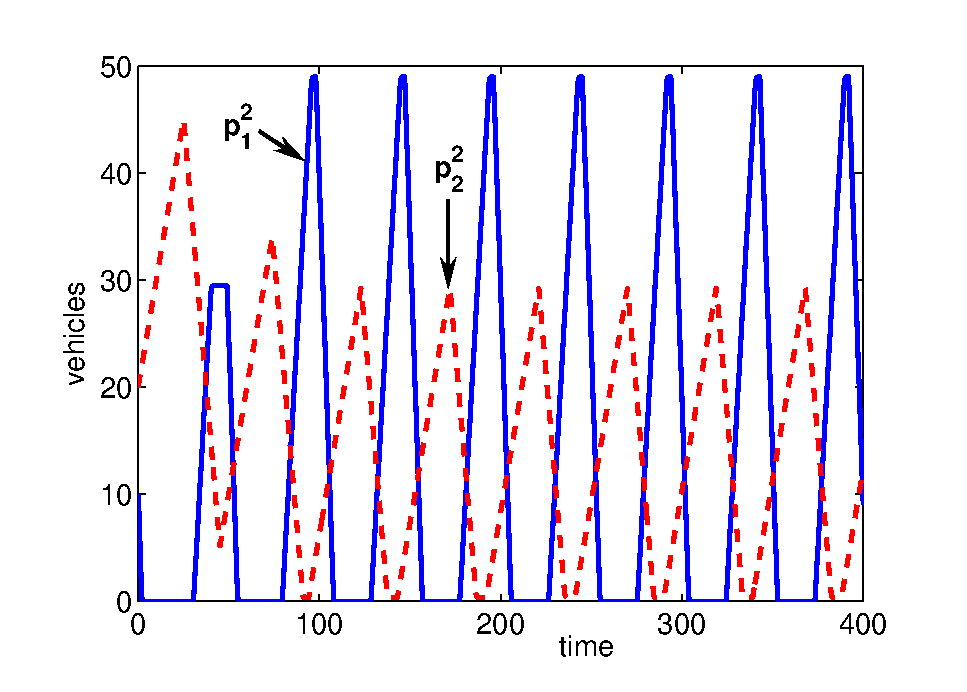
\includegraphics[width=.42\textwidth]{figs/traffic1}}
\hspace{0.5cm} \subfigure[]{
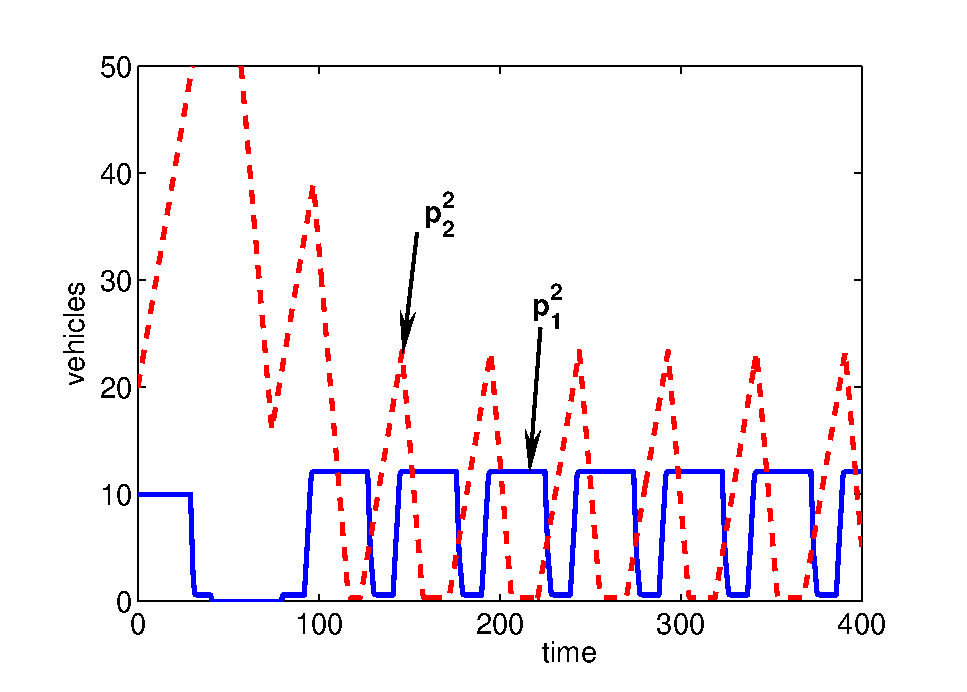
\includegraphics[width=.42\textwidth]{figs/traffic4}}
\caption{Queue lengths at intersection $2$ obtained with delays for
$\{t_5^2,t_7^2,t_9^2\}$ as  a) $\{20,20,0.1\}$ and b)
$\{14,26,29\}$. } \label{ftraficsim}
\end{figure*}

The goal in this example is to obtain, through simulations, suitable
switching delays for the second traffic light, in order to reduce
the queue lengths at intersection $2$. The parameters to optimize
are the green periods (amber periods are fixed and equal to
$\theta_{6}^2=5$ and $\theta_{8}^2=4$), i.e., the delays of $t_5^2$,
$t_7^2$ , and the offset represented by the delay of $t_9^2$. Fig.
\ref{ftraficsim} shows the evolution of the queues for the first 400
seconds, for two cases: a) with green periods $20$ seconds
and no offset, and b) with green periods $14$ for the queue $p_1^2$
and $26$ for the queue $p_2^2$ and with an offset of $29$ seconds.
Note that the second combination of parameters provide shorter
queues. For this, the effect of the offset is very important. This
example shows that simulations based on hybrid PN models can provide
information about the optimal parameters for traffic lights
(duration of stages and offset), in order to improve the performance
in neighboring traffic intersections.


\section{A biochemical system}
\label{s:pathway}

This section presents and simulates a biochemical system modeled by continuous
Petri nets. In most chemical models, the different amounts of chemical substances are expressed
in terms of concentrations rather than as whole numbers of molecules. This implies
that the state of the system is given by a vector of real numbers, where each component
represents the concentration of a compound.
On the other hand, the dynamics
of most reactions is driven by the mass action law, what roughly implies that the
speed of a reaction is proportional to the product of the concentrations of the
reactants. These facts make continuous Petri nets under product semantics an
appealing modeling formalism for biochemical systems.

\begin{figure*}
   \centering{
   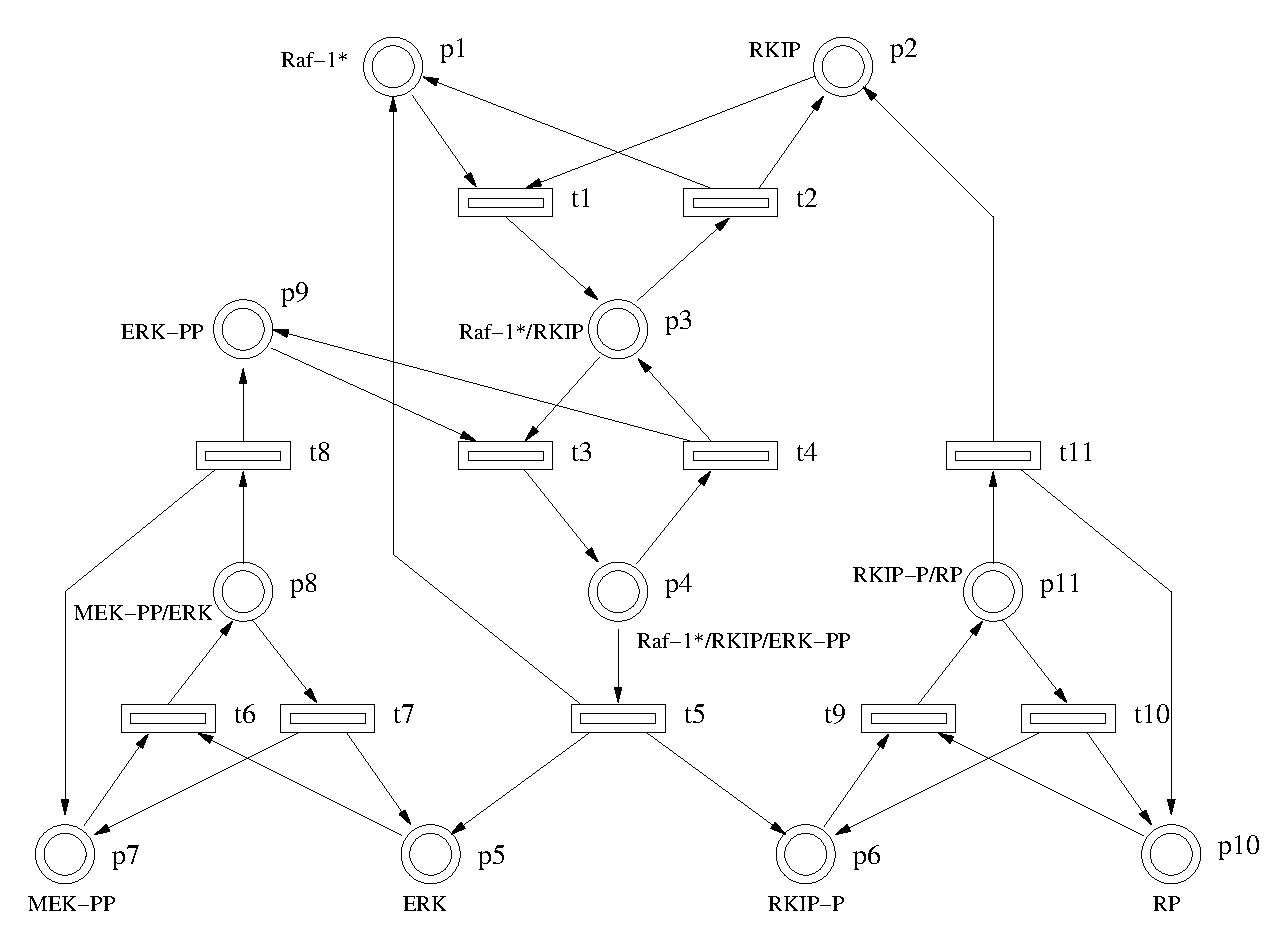
\includegraphics[width=.75\textwidth]{bioches.eps}}
   \caption{Petri net modeling the ERK signaling pathway regulated by RKIP.}
   \label{f:bioches}
\end{figure*}

The net system in Fig.~\ref{f:bioches} models a signaling pathway described and
studied in~\cite{IPChShKi03}. More precisely, the net is a graphical representation
of the Extracellular signal Regulated Kinase (ERK) signaling pathway regulated by
Raf Kinase Inhibitor Protein (RKIP). The marking of each place represents the concentration
of the compound associated to it, and the transitions represent the different
chemical reactions that take place (see~\cite{IPChShKi03} for a more detailed
description of the pathway). Notice that, although the net has conflicts, the assumed 
product semantics fully determines the flows of all continuous transitions,
and therefore it is not necessary to impose a conflict resolution policy.

Since the state of the system is expressed as concentration levels, every transition
is considered continuous and product server semantics is adopted. The parameter
$\b{\lambda}$ estimated in~\cite{IPChShKi03} is
$\b{\lambda}= [0.53,$ $0.0072,$ $0.625,$ $0.00245,$ $0.0315,$ $0.8,$ $0.0075,$ $0.071,$ $0.92,$ $0.00122,$ $0.87]$.
As initial concentrations of the compounds we take the following values:
$\mo=[2,\ 2.5,\ 0,\ 0,\ 0,\ 0,\ 2.5,\ 0,\ 2.5,\ 3,\ 0]$.

\begin{figure}
   \centering{
   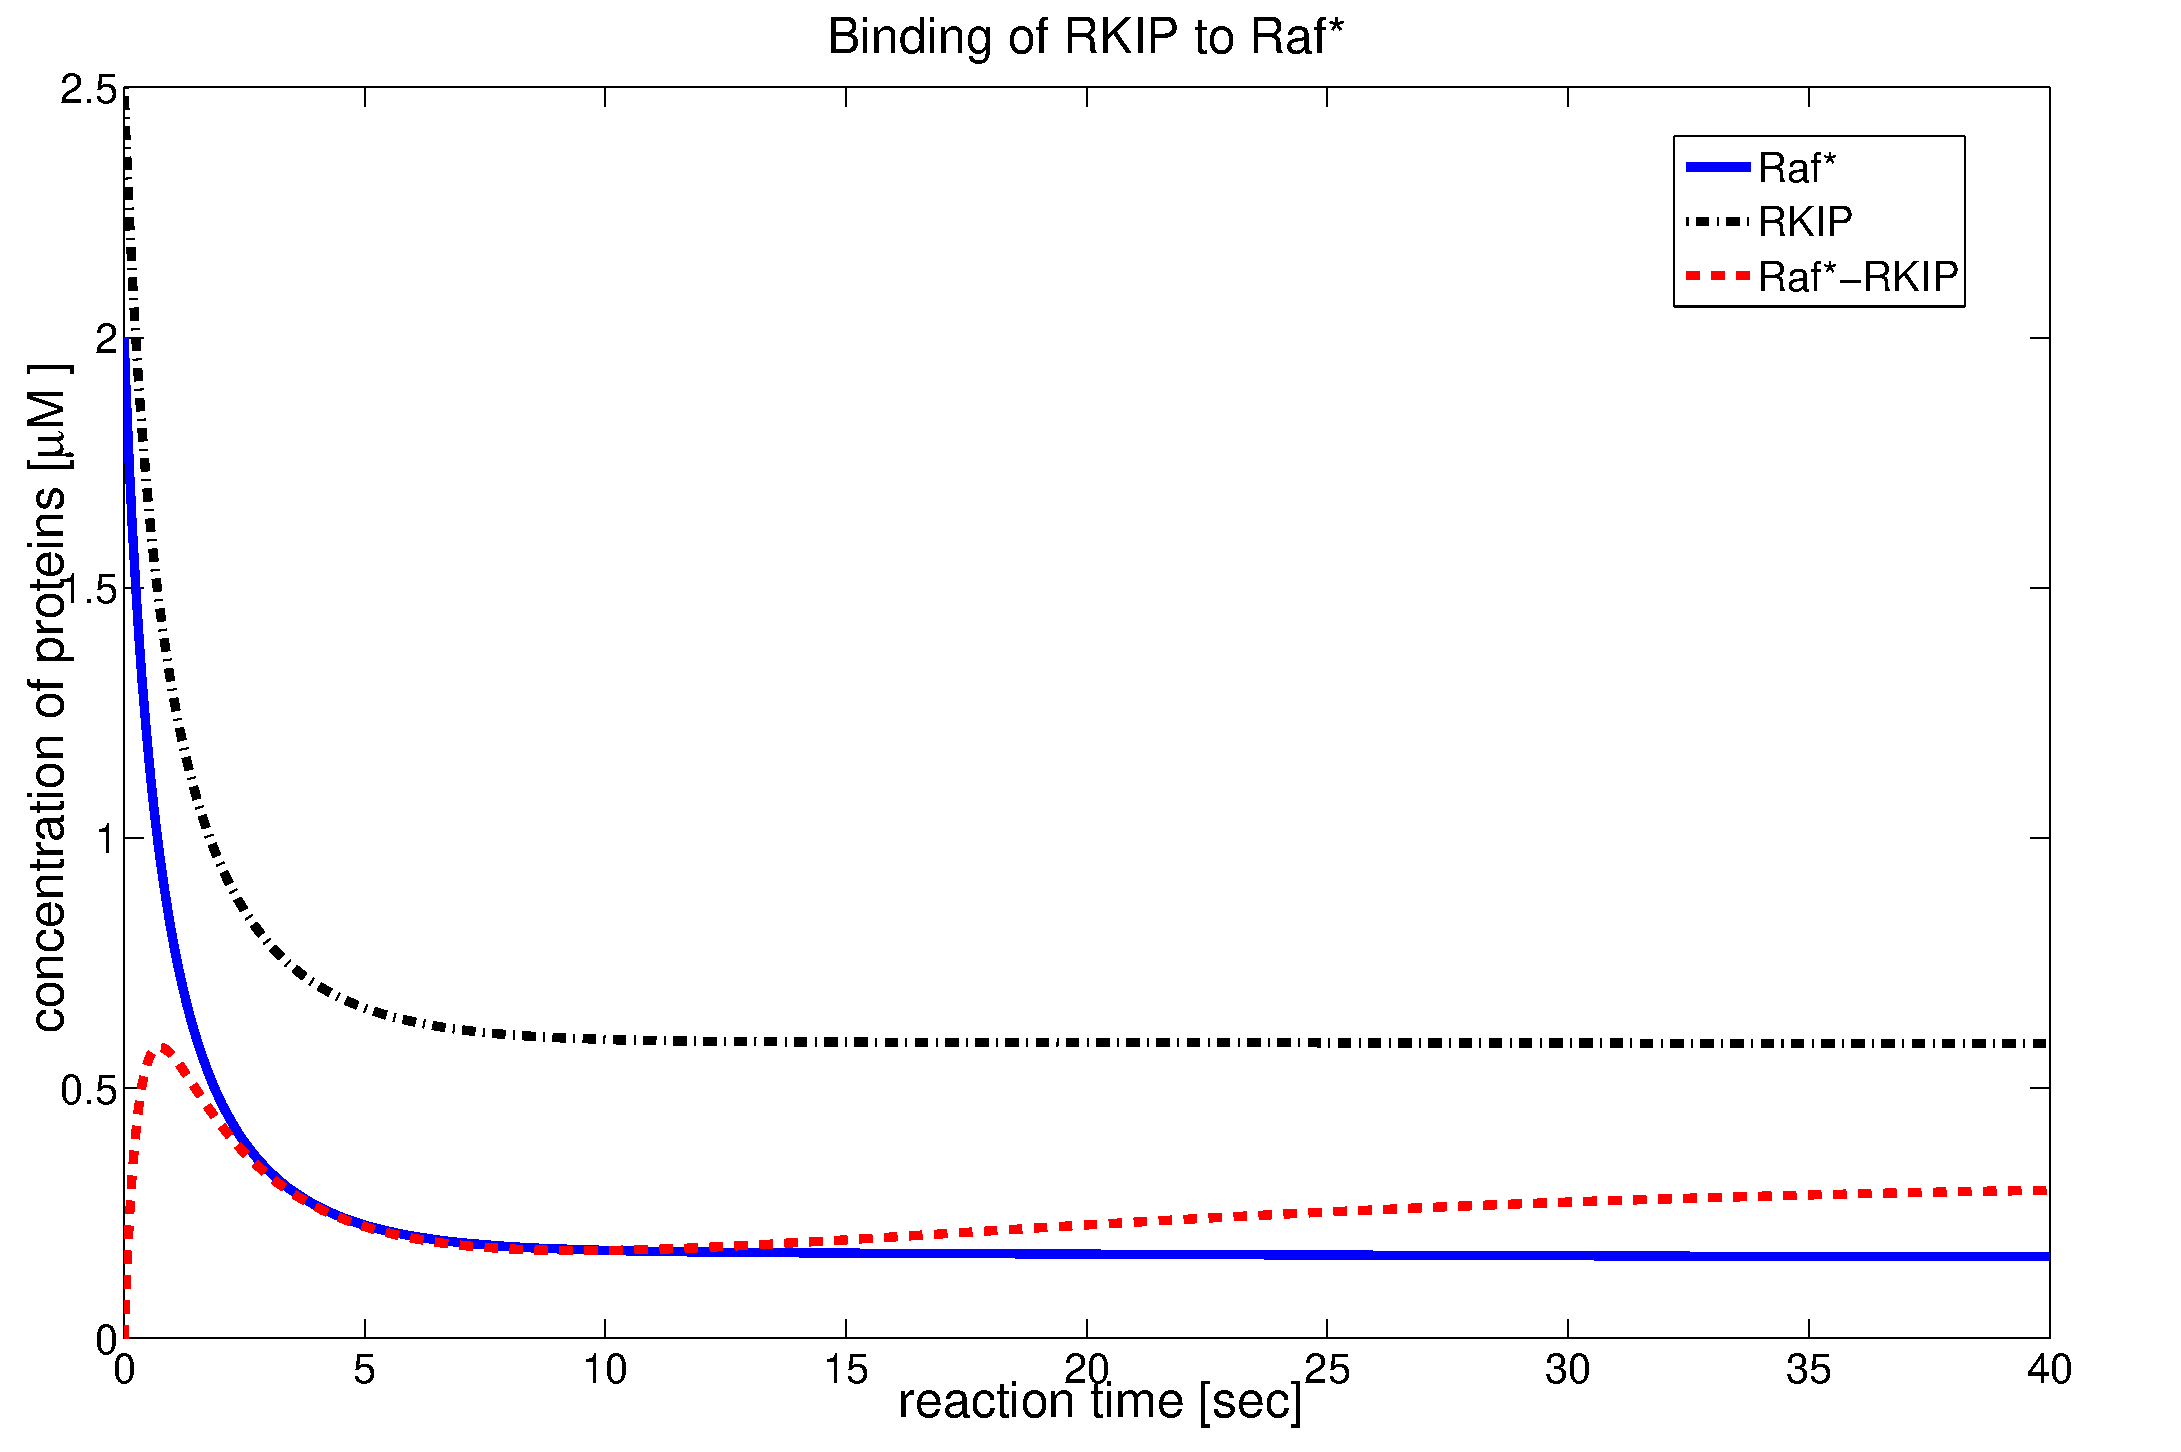
\includegraphics[width=.7\columnwidth]{mf1c1.eps}}
   \caption{Time evolution of Raf-1*, RKIP and their complex Raf-1*/RKIP.}
   \label{f-mf1c1}
\end{figure}

\begin{figure}
   \centering{
   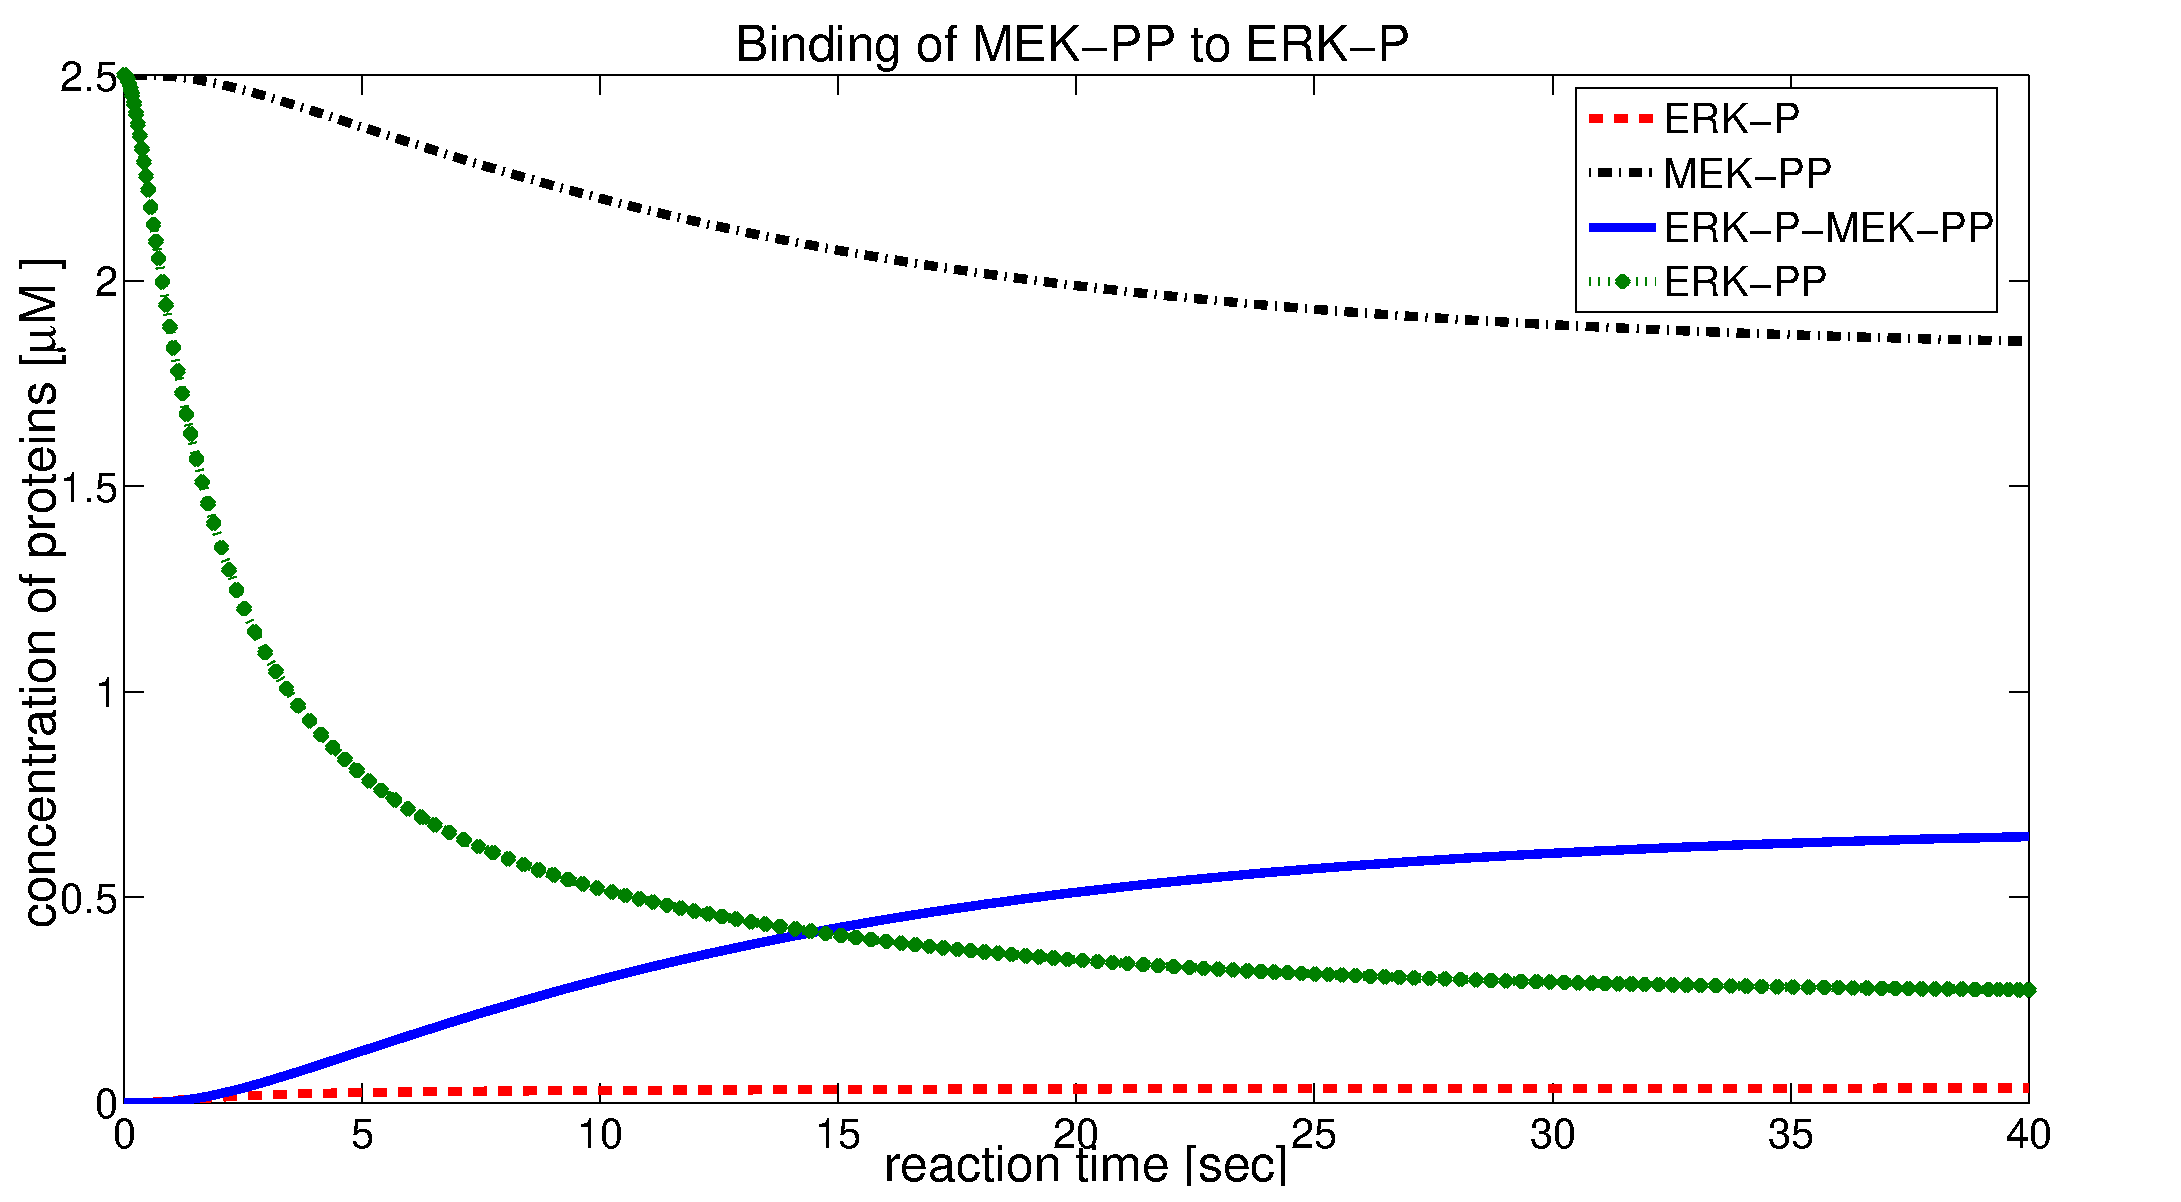
\includegraphics[width=.7\columnwidth, height=6cm]{mf1c2.eps}}
   \caption{Activity of MEK-PP which phosphorylates and activates ERK.}
   \label{f-mf1c2}
\end{figure}

Figures~\ref{f-mf1c1} and ~\ref{f-mf1c2} show the time evolution of some
of the compounds in the system along $40$ time units. In particular, Fig.~\ref{f-mf1c1}
shows the dynamics of Raf-1*, RKIP and their complex Raf-1*/RKIP, and
Fig.~\ref{f-mf1c2} shows the activity of MEK-PP which phosphorylates and activates ERK.
As discussed in~\cite{IPChShKi03}, intensive simulations can be used to
perform sensitivity analysis with respect to the variation of initial conditions.




%%%%%%%%%%%%%%%%%%%%%%%%%%%%%

\section{A Kanban-like flexible manufacturing system}


Here, we consider the Kanban-like flexible manufacturing system (FMS) consisting of two workflows that are attended by a pool of three machines (see Fig. \ref{fig:layoutFINAL}), to perform a structural controllability analysis. A TCPN that models the system is presented in Fig. \ref{fig:FMSPN} (this model is available in the models folder as Model\_FMS\_3.mat). It has 216 configurations and 11 transitions, each one representing one of the following events:
\begin{itemize}
    \item Loading of material to the machines ($t_1,t_3,t_5,t_7,t_9$).
    \item Unloading of the processed material to be stored in a buffer ($t_2,t_4,t_6,t_8,t_{10}$).
    \item Removing parts from the system output ($t_{11}$).
\end{itemize}
The timing of the net is given by $\lambda = \left [1 \ \frac{1}{3} \ 1 \ \frac{1}{4} \ 1 \ \frac{1}{3} \ 1 \ \frac{1}{5} \ 1 \ \frac{1}{5} \ 1 \right ]^T$. 
We work based on the assumption that machines are consistently working at their nominal speed and are freed up as soon as the material is processed. As a result, we have identified $T_{nc}=\{t_2,t_4,t_6,t_8,t_{10}\}$. The remaining events are controllable because it is possible to decide when to use a specific machine to process a particular piece, and we can always empty the output buffer. This leads to $T_c$ being $T_{c}=\{t_1,t_3,t_5,t_7,t_{9},t_{11}\}$.

\begin{figure}[htbp]
    \centering
    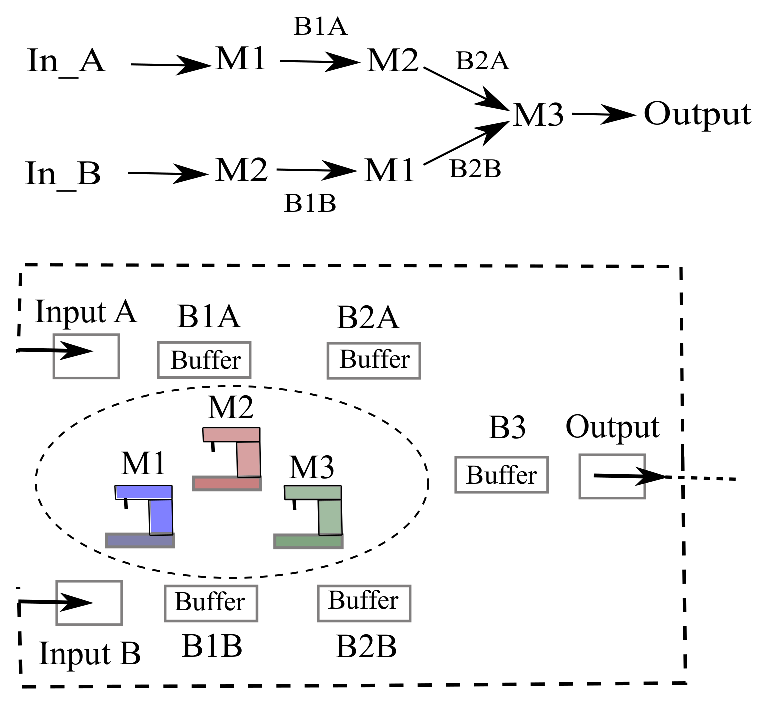
\includegraphics[scale=.6]{figs/FinalExampleLayout2.eps}
    \caption{A Kanban-like flexible manufacturing system. and its production process.}
    \label{fig:layoutFINAL}
\end{figure}

\begin{figure}[htbp]
    \centering
    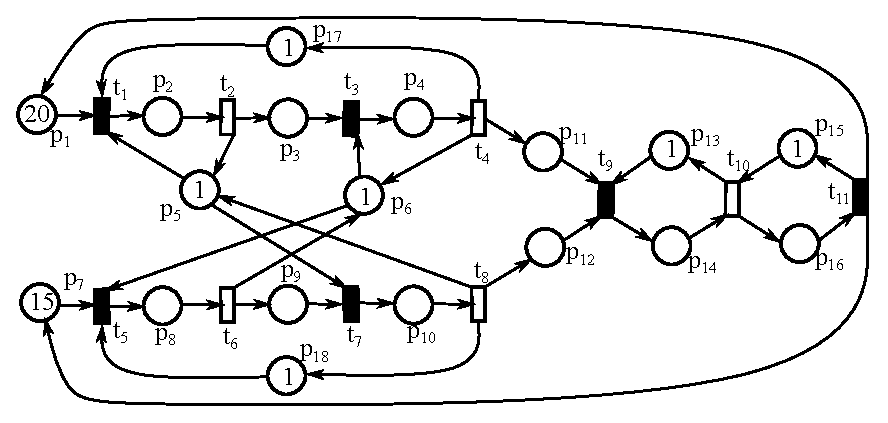
\includegraphics[scale=.75]{figs/FMS.eps}
    \caption{A TCPN system that models the FMS of Fig \ref{fig:layoutFINAL}. The controllable transitions are depicted as black transitions.}
    \label{fig:FMSPN}
\end{figure}

\textbf{Net rank-controllability analysis:} Once the model has been loaded, the test can be carried out by selecting \textit{Continuous} $\rightarrow$ \textit{Structural controllability analysis} $\rightarrow$ \textit{Net rank-controllability test}. We present 3 cases:\\
${\bullet}$ $T_c = \{t_1,t_5\}$: We enter this set of controllable transitions on the pop-up windows as $[1 \ 5]$ and we obtain the message \\``\textit{Influence is not total! Therefore, the set of controllable transitions does not guarantee net rank-controllability. The only influenced nodes are:}
\textit{Places = [1 2 3 4 5 6 7 8 9 10 11 12 17 18]}
\textit{Transitions = [1 2 3 4 5 6 7 8]}'' \\This means that, since the property of influence does not hold, then there are configurations in which the net is not rank-controllable.\\
${\bullet}$ $T_c = \{t_1,t_5,t_9,t_{11}\}$ By entering this set of controllable transitions as $[1 \ 5 \ 9 \ 11]$ we obtain the message \\``\textit{It is not possible to decide if the timed net is net rank-controllable. The condition related to the choice places is not fulfilled.}''. \\In this case the test cannot conclude if the system is NRC, since one of the sufficient conditions does not hold. In particular, the one related to the choice places. This serves to give indications to the operator/researcher about where the problem may be in order to guarantee controllability.\\
${\bullet}$ $T_c = \{t_1,t_3,t_5,t_7,t_9,t_{11}\}$: Here we choose the set that we will consider in our case study, which is such that it satisfies all the structural conditions for controllability and is indicated by the message:
``\textit{The timed net is net rank-controllable.}''.

From the previous analysis, we conclude that the system is NRC. Moreover, this system is a live and bounded TCPN. Therefore, $T_c$ also guarantees that the system will be controllable over its connected sets of equilibrium markings.\\ % For instance, in [14], we have shown how to apply control laws designed for a TCPN into the corresponding Markovian Petri net system.  Once a control law has been designed for a T CP N system, it can be used for controlling the marking of the original discrete net [4


\textbf{Equilibrium connectivity graph: } This routine can be used to calculate the equilibrium connectivity graph of a system by selecting the menu \textit{Continuous} $\rightarrow$ \textit{Structural controllability analysis} $\rightarrow$ \textit{Equilibrium connectivity graph} and entering the set of controllable transitions as the input. Each node of the resulting graph represents a configuration of the system whose region contains equilibrium markings, and the edges indicate the connection between the equilibrium markings of the different regions. This provides insights into the controllability of the system, showing the sets of equilibrium points where the controllability property holds. 


Using this routine and selecting the set of controllable transitions $[1 \ 3 \ 5 \ 7 \ 9 \ 11]$, a matrix E\_conf is obtained. Each row of this matrix represents a configuration of the system in which equilibrium markings are present in the corresponding regions. For this particular case, the results are the following:


E\_conf =\\
     1     2     3     4     7     8     9    10    13    14    16   (node 1) \qquad
     1     2     3     4     7     8     9    10    13    15    16   (node 2)\\
     1     2     3     4    18     8     9    10    12    14    16 (node 3) \qquad
     1     2     3     4    18     8     9    10    12    15    16 (node 4)\\
     1     2     3     4    18     8     9    10    13    14    16 (node 5)\qquad
     1     2     3     4    18     8     9    10    13    15    16 (node 6)\\
    17     2     3     4     7     8     9    10    11    14    16 (node 7)\qquad
    17     2     3     4     7     8     9    10    11    15    16 (node 8)\\
    17     2     3     4     7     8     9    10    13    14    16 (node 9)\qquad
    17     2     3     4     7     8     9    10    13    15    16 (node 10)\\
    17     2     3     4    18     8     9    10    11    14    16 (node 11)\qquad
    17     2     3     4    18     8     9    10    11    15    16 (node 12)\\
    17     2     3     4    18     8     9    10    12    14    16 (node 13)\qquad
    17     2     3     4    18     8     9    10    12    15    16 (node 14)\\
    17     2     3     4    18     8     9    10    13    14    16 (node 15)\qquad
    17     2     3     4    18     8     9    10    13    15    16 (node 16)\\

For instance, the region corresponding to the configuration $\mathcal{C}_1 = \{(p_1,t_1),(p_2,t_2),(p_3,t_3),(p_4,t_4),(p_7,t_5),(p_8,t_6),(p_9,t_7),(p_{10},t_8),(p_{13},t_9)$, $(p_{14},t_{10}),(p_{16},t_{11})\}$ (node 1) contains equilibria. Furthermore, the routine generates a variable-type graph called E\_graph, which has 16 nodes and 76 edges, representing the connectivity of the equilibrium sets. This graph can be plotted (as in Fig. \ref{fig:my_label}), providing a visual representation of the equilibrium connectivity of the system. For this particular case, the equilibrium sets in all the regions are connected, meaning that the system exhibits the controllability property over all of its equilibrium markings. 


\begin{figure}
    \centering
    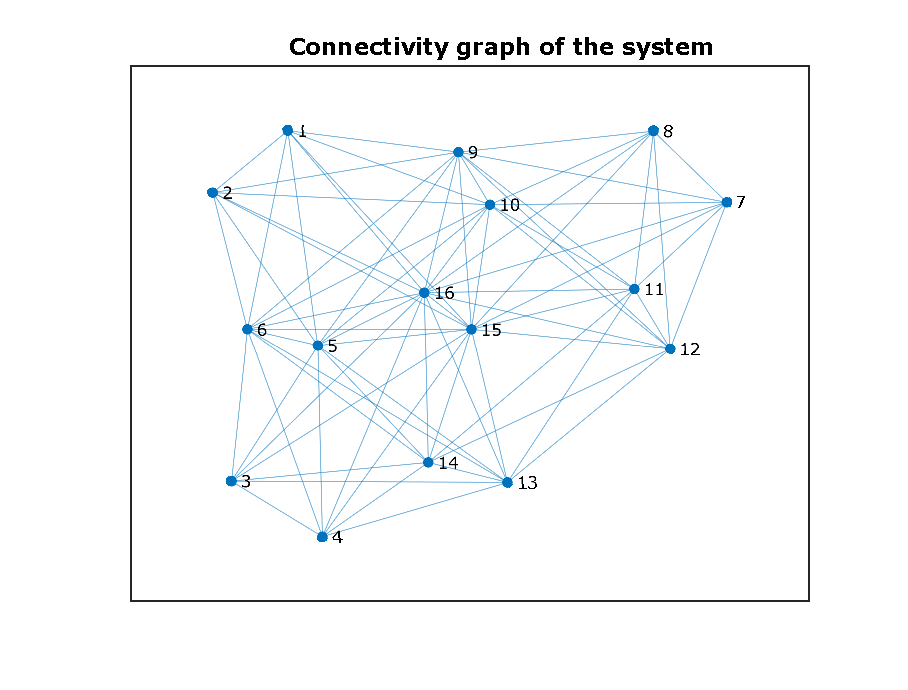
\includegraphics{figs/E_graph.eps}
    \caption{Equilibrium connectivity graph of the FMS system. Each node corresponds to a single region of the TCPN system in which it contains equilibrium markings.}
    \label{fig:my_label}
\end{figure}

%%%%%%%%%%%%%%%%%%%%%%%%%%%%%
\section{Fault Diagnosis with continuous Petri nets}
\label{sec:fdsexamps}

The following examples illustrating the fault diagnosis procedure using untimed continuous Petri nets have been considered in \cite{ARMASECASI12}. 

\subsection{Example 1}
Let us consider the Petri net in Figure~\ref{f-es1} with:
$$T_o=\{t_1, t_2, t_3 \}, \quad T_u=\{ \varepsilon_4, \varepsilon_5, \varepsilon_6, \varepsilon_7,
\varepsilon_8 \} \quad {\text and} \quad T_f^1=\{ \varepsilon_5\}.$$

\begin{figure}[]
\begin{center}
\includegraphics*[scale=.5]{fig1.eps}
\caption[]{The Petri net system considered in Examples~5, 8, 10 and
12 of \cite{ARMASECASI12}.}
   \label{f-es1}
\end{center}
\end{figure}

The matrices $Pre$, $Post$ and $m_0$ can be imported in $SimHPN$ toolbox using
$diagnosis1.mat$ file from the $Models$ folder. Places and transitions follow the
numeration in Figure~\ref{f-es1}. The following input parameters should be used:

\begin{itemize}
\item Number of observable transitions: $3$
\item Sequence of observed transitions: $[ 1 \ 2 \ 3 ]$
\item Sequence of observed firing quantity of transitions: $[0.7 \ 0.5 \ 0.5]$
\item Number of fault classes: $1$
\item Transitions in fault class $1$: $5$
\end{itemize}

In such a case we have only one fault class containing transition
$\varepsilon_5$. Note that, in the matrices $Pre$ and $Post$ the observable transitions have to
occupy the first columns. We are considering the following
observation: $t_1(0.7) t_2(0.5) t_3(0.5)$. The following results are shown at the MATLAB command prompt:

\begin{verbatim}
Number of observable transitions: 3 
First 3 transitions are observable and the rest not
Fault class Tf^{1}={\epsilon_5}

Observed sequence: t1(0.7)t2(0.5)t3(0.5) 
=========================================
==========press a key to continue========
=========================================

Enabling bound of t4 is 2
Enabling bound of t5 is 2
Enabling bound of t6 is 2
Enabling bound of t7 is 2
Enabling bound of t8 is 2

***********************************************************
For empty word:
***********************************************************

Vertices of the set of consistent markings (vertices of \bar Y(m_0,w))
e_1 = [0 1 0 0 0 0 1 0 0 0 0 0]'
e_2 = [0 0 1 0 1 0 1 0 0 1 0 0]'

Computing the diagnosis states
Diagnosis state for Tf^{1}: N

***********************************************************
Observed sequence:  t1(0.70)
***********************************************************

Vertices of the set of consistent markings after cutting
e_1 = [0 0.3 0.7 0 0.7 0 1 0 0 0.7 0 0]'
e_2 = [0 0 1 0 1 0 1 0 0 1 0 0]'
***********************************************************
Vertices of the set of consistent markings (vertices of \bar Y(m_0,w))
e_1 = [0 0 0.3 0 0.3 0 1.7 0 0 1 0 0.7]'
e_2 = [0 0.3 0 0 0 0 1.7 0 0 0.7 0 0.7]'
e_3 = [0 0.3 0 0 0 0.7 1 0 0 0.7 0 0]'
e_4 = [0 0 0.3 0 0.3 0.7 1 0 0 1 0 0]'
Computation time:                 0.01 seconds
Computing the diagnosis states
Diagnosis state for Tf^{1}: N

***********************************************************
Observed sequence:  t1(0.70) t2(0.50)
***********************************************************

Vertices of the set of consistent markings after cutting
e_1 = [0 0.3 0 0 0 0 1.7 0 0 0.7 0 0.7]'
e_2 = [0 0 0.3 0 0.3 0 1.7 0 0 1 0 0.7]'
e_3 = [0 0 0.3 0 0.3 0.7 1 0 0 1 0 0]'
e_4 = [0 0.3 0 0 0 0.7 1 0 0 0.7 0 0]'
***********************************************************
Vertices of the set of consistent markings (vertices of \bar Y(m_0,w))
e_1 = [0 0.3 0.5 0 0.5 0 1.2 0 0.5 0.7 0.5 0.7]'
e_2 = [0.5 0.3 0 0 0 0 1.2 0 0 0.7 0 0.7]'
e_3 = [0 0.3 0.5 0.5 0 0 1.2 0 0.5 0.7 0 0.7]'
e_4 = [0 0.8 0 0 0 0 1.2 0.5 0 0.7 0 0.7]'
e_5 = [0 0 0.8 0 0.8 0 1.2 0.5 0 1.5 0 0.7]'
e_6 = [0 0 0.8 0.5 0.3 0 1.2 0 0.5 1 0 0.7]'
e_7 = [0.5 0 0.3 0 0.3 0 1.2 0 0 1 0 0.7]'
e_8 = [0 0 0.8 0 0.8 0 1.2 0 0.5 1 0.5 0.7]'
e_9 = [0 0 0.8 0 0.8 0.7 0.5 0.5 0 1.5 0 0]'
e_10 = [0 0 0.8 0.5 0.3 0.7 0.5 0 0.5 1 0 0]'
e_11 = [0.5 0 0.3 0 0.3 0.7 0.5 0 0 1 0 0]'
e_12 = [0 0 0.8 0 0.8 0.7 0.5 0 0.5 1 0.5 0]'
e_13 = [0 0.8 0 0 0 0.7 0.5 0.5 0 0.7 0 0]'
e_14 = [0 0.3 0.5 0.5 0 0.7 0.5 0 0.5 0.7 0 0]'
e_15 = [0.5 0.3 0 0 0 0.7 0.5 0 0 0.7 0 0]'
e_16 = [0 0.3 0.5 0 0.5 0.7 0.5 0 0.5 0.7 0.5 0]'
Computation time:                 0.01 seconds
Computing the diagnosis states
Diagnosis state for Tf^{1}: U

***********************************************************
Observed sequence:  t1(0.70) t2(0.50) t3(0.50)
***********************************************************

Vertices of the set of consistent markings after cutting
e_1 = [0 0.3 0.5 0.5 0 0 1.2 0 0.5 0.7 0 0.7]'
e_2 = [0 0 0.8 0.5 0.3 0 1.2 0 0.5 1 0 0.7]'
e_3 = [0 0 0.8 0.5 0.3 0.7 0.5 0 0.5 1 0 0]'
e_4 = [0 0.3 0.5 0.5 0 0.7 0.5 0 0.5 0.7 0 0]'
***********************************************************
Vertices of the set of consistent markings (vertices of \bar Y(m_0,w))
e_1 = [0 0 0.8 0 0.3 0 1.2 0 0.5 1 0 0.7]'
e_2 = [0 0.3 0.5 0 0 0 1.2 0 0.5 0.7 0 0.7]'
e_3 = [0 0.3 0.5 0 0 0.7 0.5 0 0.5 0.7 0 0]'
e_4 = [0 0 0.8 0 0.3 0.7 0.5 0 0.5 1 0 0]'
Computation time:                 0.00 seconds
Computing the diagnosis states
Diagnosis state for Tf^{1}: F
\end{verbatim}

\subsection{Example 2: (a manufacturing system)}

Let us consider the Petri net in Fig.~\ref{model2} where transitions
$t_1$ to $t_{12}$ correspond to observable events, transitions
$\varepsilon_{13}$ to $\varepsilon_{24}$ correspond to unobservable
but regular events while $\varepsilon_{25}$ and $\varepsilon_{26}$
are unobservable and faulty transitions. In particular we assume
$T_f^1=\{\varepsilon_{25}\}$ and $T_f^2=\{\varepsilon_{26}\}$.

\begin{figure*}
\begin{center}
\includegraphics*[scale=0.7]{manufacturing.eps}
\end{center}
\caption{Petri net model of the manufacturing system considered in
Subsection~VII.A.} \label{model2}
\end{figure*}

The matrices $Pre$, $Post$ and $m_0$ are defined in the MATLAB file
$Diagnosis\_2.mat$ and can be imported in $SimHPN$ toolbox using the menu $File\ \rightarrow \ Import\ from\ .mat\ file$. Places and transitions follow the numeration in Fig.~\ref{model2}. The following parameters will be considered:

\begin{itemize}
\item Number of observable transitions: $12$
\item Sequence of observed transitions: $[1  \   1  \   2  \  12 \    3 \    12 \    3  \   6 \    7 \    8  \   4   \  5 \    9\    10  \  11 ]$
\item Sequence of observed firing quantity of transitions: $[1  \   1 \    1 \    1   \  1    \ 1  \   1 \    1  \   1  \   1   \  1  \   1  \   1  \   1 \    1]$
\item Number of fault classes: $1$
\item Transitions in fault class $1$: $[25\ 26]$
\end{itemize}

This net system has two fault classes. The first one contains transition
$\varepsilon_{25}$ and the second one contains transition
$\varepsilon_{26}$. The cardinality of the set of observable
transitions is $12$ and the considered observation is $w= t_1(1)
t_1(1) t_2(1) t_{12}(1) t_3(1) t_{12}(1) t_3(1) t_6(1) t_7(1)t_8(1)
t_4(1) t_5(1) t_9(1) t_{10}(1) t_{11}(1)$. The fault state after each observation is shown at the MATLAB command prompt.

\subsection{Example 3: (unobservable acyclic subnet)}

Let us consider the Petri net in Figure~\ref{fig_new_example2} where
transitions $t_1$ to $t_{6}$ correspond to observable events,
transitions $\varepsilon_{7}$ and $\varepsilon_{8}$ correspond to
unobservable but regular events while $\varepsilon_{9}$ and
$\varepsilon_{10}$ are unobservable and faulty transitions. In
particular we assume $T_f^1=\{\varepsilon_{9}\}$ and
$T_f^2=\{\varepsilon_{10}\}$.

\begin{figure}
\begin{center}
\includegraphics*[scale=0.6]{example2.eps}
\end{center}
\caption{The Petri net considered in Subsection~VII.B.}
\label{fig_new_example2}
\end{figure}

The matrices $Pre$, $Post$ and $m_0$ can be imported from
$Diagnosis\_3.mat$ file. Places and transitions follow the
numeration in Fig.~\ref{model2} and the following parameters are used:

\begin{itemize}
\item Number of observable transitions: $6$
\item Sequence of observed transitions: $[1  \   2  \   5  \  4 \    1 \    3 ]$
\item Sequence of observed firing quantity of transitions: $[0.1   \ 0.1  \  0.3  \  0.1  \ 0.1  \  0.1]$
\item Number of fault classes: $2$
\item Transitions in fault class $1$: $[9]$
\item Transitions in fault class $2$: $[10]$
\end{itemize}


Such net has two fault classes. The first one contains transition
$\varepsilon_{9}$ and the second one contains transition
$\varepsilon_{10}$. The cardinality of the set of observable
transitions is $6$ and the considered observation is $w= t_1(0.1)
t_2(0.1) t_5(0.3) t_{4}(0.1) t_1(0.1) t_{3}(0.1)$. The following
results are obtained at the MATLAB prompt:



\begin{verbatim}
Number of observable transitions: 6 
First 6 transitions are observable and the rest not
Fault class Tf^{1}={\epsilon_9}
Fault class Tf^{2}={\epsilon_10}

Observed sequence: t1(0.1)t2(0.1)t5(0.3)t4(0.1)t1(0.1)t3(0.1) 
=========================================
==========press a key to continue========
=========================================

Enabling bound of t7 is 2.000000e+00
Enabling bound of t8 is 2.000000e+00
Enabling bound of t9 is 2
Enabling bound of t10 is 2.000000e+00

***********************************************************
For empty word:
***********************************************************

Vertices of the set of consistent markings (vertices of \bar Y(m_0,w))
e_1 = [2 2 0 0 0 0 0 0 0 0 0 0]'

Computing the diagnosis states
Diagnosis state for Tf^{1}: N
Diagnosis state for Tf^{2}: N

***********************************************************
Observed sequence:  t1(0.10)
***********************************************************

Vertices of the set of consistent markings after cutting
e_1 = [2 2 0 0 0 0 0 0 0 0 0 0]'
***********************************************************
Vertices of the set of consistent markings (vertices of \bar Y(m_0,w))
e_1 = [1.6 2 0 0 0 0 0.2 0 0.1 0 0.1 0]'
e_2 = [1.6 2 0.1 0 0 0 0.1 0 0.1 0 0 0]'
e_3 = [1.6 2 0.1 0.1 0 0 0 0 0 0 0 0]'
e_4 = [1.6 2 0 0.1 0 0 0.1 0 0 0 0.1 0]'
Computation time:                 0.01 seconds
Computing the diagnosis states
Diagnosis state for Tf^{1}: U
Diagnosis state for Tf^{2}: N

***********************************************************
Observed sequence:  t1(0.10) t2(0.10)
***********************************************************

Vertices of the set of consistent markings after cutting
e_1 = [1.6 2 0.1 0 0 0 0.1 0 0.1 0 0 0]'
e_2 = [1.6 2 0 0 0 0 0.2 0 0.1 0 0.1 0]'
e_3 = [1.6 2 0 0.1 0 0 0.1 0 0 0 0.1 0]'
e_4 = [1.6 2 0.1 0.1 0 0 0 0 0 0 0 0]'
***********************************************************
Vertices of the set of consistent markings (vertices of \bar Y(m_0,w))
e_1 = [1.6 1.6 0 0.1 0 0.1 0.2 0 0 0.1 0.1 0]'
e_2 = [1.6 1.6 0.1 0.1 0 0.1 0.1 0 0 0.1 0 0]'
e_3 = [1.6 1.6 0.1 0 0 0.1 0.2 0 0.1 0.1 0 0]'
e_4 = [1.6 1.6 0 0 0 0.1 0.3 0 0.1 0.1 0.1 0]'
e_5 = [1.6 1.6 0.1 0 0.1 0.1 0.1 0 0.1 0 0 0]'
e_6 = [1.6 1.6 0 0 0.1 0.1 0.2 0 0.1 0 0.1 0]'
e_7 = [1.6 1.6 0.1 0 0 0.2 0.1 0 0.1 0 0 0.1]'
e_8 = [1.6 1.6 0 0 0 0.2 0.2 0 0.1 0 0.1 0.1]'
e_9 = [1.6 1.6 0.1 0.1 0.1 0.1 0 0 0 0 0 0]'
e_10 = [1.6 1.6 0 0.1 0.1 0.1 0.1 0 0 0 0.1 0]'
e_11 = [1.6 1.6 0.1 0.1 0 0.2 0 0 0 0 0 0.1]'
e_12 = [1.6 1.6 0 0.1 0 0.2 0.1 0 0 0 0.1 0.1]'
Computation time:                 0.01 seconds
Computing the diagnosis states
Diagnosis state for Tf^{1}: U
Diagnosis state for Tf^{2}: U

***********************************************************
Observed sequence:  t1(0.10) t2(0.10) t5(0.30)
***********************************************************

Vertices of the set of consistent markings after cutting
e_1 = [1.6 1.6 0 0 0 0.1 0.3 0 0.1 0.1 0.1 0]'
***********************************************************
Vertices of the set of consistent markings (vertices of \bar Y(m_0,w))
e_1 = [1.9 1.9 0 0 0 0.1 0 0 0.1 0.1 0.1 0]'
Computation time:                 0.00 seconds
Computing the diagnosis states
Diagnosis state for Tf^{1}: F
Diagnosis state for Tf^{2}: N

***********************************************************
Observed sequence:  t1(0.10) t2(0.10) t5(0.30) t4(0.10)
***********************************************************

Vertices of the set of consistent markings after cutting
e_1 = [1.9 1.9 0 0 0 0.1 0 0 0.1 0.1 0.1 0]'
***********************************************************
Vertices of the set of consistent markings (vertices of \bar Y(m_0,w))
e_1 = [1.9 1.9 0 0 0 0 0 0.1 0.1 0.1 0.1 0]'
Computation time:                 0.00 seconds
Computing the diagnosis states
Diagnosis state for Tf^{1}: F
Diagnosis state for Tf^{2}: N

***********************************************************
Observed sequence:  t1(0.10) t2(0.10) t5(0.30) t4(0.10) t1(0.10)
***********************************************************

Vertices of the set of consistent markings after cutting
e_1 = [1.9 1.9 0 0 0 0 0 0.1 0.1 0.1 0.1 0]'
***********************************************************
Vertices of the set of consistent markings (vertices of \bar Y(m_0,w))
e_1 = [1.5 1.9 0 0 0 0 0.2 0.1 0.2 0.1 0.2 0]'
e_2 = [1.5 1.9 0.1 0 0 0 0.1 0.1 0.2 0.1 0.1 0]'
e_3 = [1.5 1.9 0.1 0.1 0 0 0 0.1 0.1 0.1 0.1 0]'
e_4 = [1.5 1.9 0 0.1 0 0 0.1 0.1 0.1 0.1 0.2 0]'
Computation time:                 0.00 seconds
Computing the diagnosis states
Diagnosis state for Tf^{1}: F
Diagnosis state for Tf^{2}: N

***********************************************************
Observed sequence:  t1(0.10) t2(0.10) t5(0.30) t4(0.10) t1(0.10) t3(0.10)
***********************************************************

Vertices of the set of consistent markings after cutting
e_1 = [1.5 1.9 0.1 0 0 0 0.1 0.1 0.2 0.1 0.1 0]'
e_2 = [1.5 1.9 0.1 0.1 0 0 0 0.1 0.1 0.1 0.1 0]'
***********************************************************
Vertices of the set of consistent markings (vertices of \bar Y(m_0,w))
e_1 = [1.5 1.9 0 0 0 0 0.1 0.2 0.2 0.1 0.1 0]'
e_2 = [1.5 1.9 0 0.1 0 0 0 0.2 0.1 0.1 0.1 0]'
Computation time:                 0.00 seconds
Computing the diagnosis states
Diagnosis state for Tf^{1}: F
Diagnosis state for Tf^{2}: N
\end{verbatim}

\newpage


% --- BIBLIOGRAFIA -------------------------------------------------------

%\backmatter
%\pagestyle{fancy}

%\input{RelevantPublications.bbl}%Fichero creado a mano desde Thesis.bbl

%paginacion Bibliografia: modificar a mano Thesis.toc y compilar con \nofiles

%\renewcommand{\bibname}{Bibliography}

\bibliographystyle{alpha}
\addcontentsline{toc}{chapter}{\bibname}
\bibliography{et}

%-- INDICE DE TERMINOS ----------------------------------------------------

%\addcontentsline{toc}{chapter}{\indexname}
%\printindex

\end{document}
